\documentclass[fleqn,10pt]{wlscirep}
\usepackage[utf8]{inputenc}
\usepackage[T1]{fontenc}
\usepackage{amsmath,amssymb}
\usepackage{booktabs}
\usepackage{multirow}
\usepackage{microtype}
\usepackage{xcolor}
\usepackage{graphicx}
\usepackage{enumitem}
\usepackage{amsthm}
\usepackage{listings}
\lstset{basicstyle=\ttfamily\scriptsize,breaklines=true,columns=fullflexible,
        frame=single,framesep=3pt,xleftmargin=3pt,aboveskip=4pt,belowskip=2pt,
        breakindent=0pt,keepspaces=true}
\newtheorem{definition}{Definition}

% -----------------------------------------------------------------------
%  Helpers for draft: shaded placeholder boxes for figures
% -----------------------------------------------------------------------
\usepackage{mdframed}
\newcommand{\figplaceholder}[2][9cm]{%
  \begin{mdframed}[backgroundcolor=gray!12,linecolor=gray!40,linewidth=0.6pt]%
  \centering\vspace{0.4cm}%
  \textcolor{gray!70}{\small\textit{#2}}%
  \vspace{0.4cm}%
  \end{mdframed}}

% -----------------------------------------------------------------------
\title{Forecasting Through Meteorological Reasoning:\\
       When Language Models Materialize a World Model of Precipitation Physics}

\author[1,*]{[Author One]}
\author[1]{[Author Two]}
\affil[1]{[Affiliation, Department, City, Country]}
\affil[*]{[corresponding@email.example]}

\keywords{%
  precipitation nowcasting;
  vision-language models;
  world models;
  information bottleneck;
  interpretable machine learning;
  atmospheric physics}

\begin{abstract}
Short-range precipitation nowcasting fails most severely during convective initiation and rapid growth---the regimes in which a brief radar history admits many physically distinct futures, in which a skilful warning matters most, and whose frequency is rising under climate change.
State-of-the-art deep-learning nowcasters resolve this ambiguity inside opaque latent representations that a forecaster can neither read nor correct, and physics-informed variants inject only governing equations, leaving the seasonal, geographic, diurnal, and synoptic knowledge that human forecasters depend on unrepresented.
Here we introduce the Atmospheric Scene Graph World Model (ASG-WM), which forecasts \emph{through} an explicit, human-readable world state rather than around a hidden one.
A vision--language model reads a multi-channel radar--satellite sequence and, with no human-supplied text at inference, constructs the Atmospheric Scene Graph---a constrained-grammar state of storm objects carrying positions, motion vectors, growth--decay tendencies, regime labels, and per-attribute uncertainty.
A physics-informed renderer then materialises the forecast field from this predicted state and a future-blind advection of the present, and from nothing else.
This architectural information bottleneck makes the structured state the sole causal path to the forecast, so faithfulness is not asserted but entailed: zeroing the scene graph provably collapses the forecast to advection, and editing a storm object changes the forecast exactly as the state dictates.
We formalise this notion of architectural faithfulness, specify a test suite that probes causality directly rather than through post-hoc saliency, and design a regime-stratified evaluation against twelve baselines on the SEVIR benchmark alongside a five-category ablation of meteorological knowledge---governing equations, seasonal, geographic, diurnal, and synoptic priors---each with a matched held-out test.
ASG-WM reframes interpretability in physical forecasting from a property one hopes to observe into one the architecture guarantees, offering a template for faithful, intervenable world models wherever prediction is governed by partial physical knowledge.
\end{abstract}

\begin{document}
\flushbottom
\maketitle
\thispagestyle{empty}

% ===================================================================
\section*{Introduction}
% ===================================================================

Short-range precipitation forecasting over the 0--3\,h horizon---nowcasting---is among the most operationally consequential tasks in meteorology.
Accurate nowcasts underpin flash-flood warnings, aviation weather advisories, urban-drainage management, and severe-convective alerting.
The 0--3\,h window is a niche where numerical weather prediction (NWP) struggles because the governing convective processes occur at sub-NWP grid scales, yet the observation record is long enough in principle to constrain the immediate future.
The events that matter most---convective initiation and rapid growth---are also where nowcasting fails most often: a brief radar history is consistent with many physically distinct futures, and resolving that ambiguity requires meteorological reasoning rather than kinematic extrapolation.
These same high-impact events are becoming more frequent and intense under observed and projected climate change~\cite{ipcc2021ar6}, sharpening the need for nowcasting systems whose skill on the ambiguous, dangerous cases can be both improved and \emph{trusted}.

Deep learning has transformed nowcasting skill over the past decade, with recurrent~\cite{shi2015convlstm,shi2017trajgru,wang2017predrnn,wang2018predrnnpp}, convolutional~\cite{ayzel2020rainnet,trebing2021smaatunet}, transformer~\cite{gao2022earthformer,sonderby2020metnet,espeholt2022metnet2}, and generative~\cite{ravuri2021dgmr,zhang2023nowcastnet,leinonen2023ldcast,gao2023prediff,yu2024diffcast,gong2024cascast} architectures each advancing the state of the art.
Leading generative nowcasters achieve high skill by encoding radar history into high-dimensional latent representations and sampling probabilistic futures; NowcastNet~\cite{zhang2023nowcastnet} even embeds advection and continuity constraints into its evolution network.
Yet in every case the internal state driving the prediction is a dense, opaque latent vector: a forecaster cannot ask the model which cell is growing and why, revise that belief, and watch the forecast respond.
The motivating axis for this work is therefore not ``physics versus no physics''---NowcastNet already embeds governing equations---but \emph{hidden state versus an explicit, human-readable, manipulable state}.
We argue that an interpretable and \emph{intervenable} world model is the more consequential target, because it is what makes a forecast both improvable on the hard regimes and inspectable by the forecaster who must act on it.

Casting the problem as ``physics-informed'' is, moreover, narrower than commonly recognised.
Existing physics-informed nowcasters inject one class of physical knowledge---governing \emph{equations}: the advection PDE, mass-conservation constraints, and convective-stability criteria.
Operational forecasting depends on at least four additional knowledge types that PDEs alone cannot encode (Figure~\ref{fig:knowledge}):
\emph{seasonal priors} (deep-moist convection concentrates in the warm season when CAPE is plentiful; cool-season precipitation is predominantly stratiform);
\emph{geographic context} (orographic lift, coastal sea-breeze convergence, and urban heat islands trigger convection at reproducible positions);
\emph{diurnal forcing} (afternoon surface heating, nocturnal low-level jets sustaining mesoscale convective systems);
and \emph{synoptic pattern recognition} (frontal positions, drylines, jet placement, and moisture transport that decide whether initiating convection organises into a hazardous system).
None of these reduces to a PDE; they are contextual, relational, and climatologically conditioned, and acquiring them requires a model that has \emph{learned} meteorological knowledge, not one merely handed equations at training time.
The initiation and growth regimes where this non-equation knowledge is most decisive are exactly where nowcasting most often fails---so closing the gap between equation-informed and more fully meteorologically-informed prediction is, we argue, where the operational payoff is largest.

\begin{figure*}[ht]
\centering
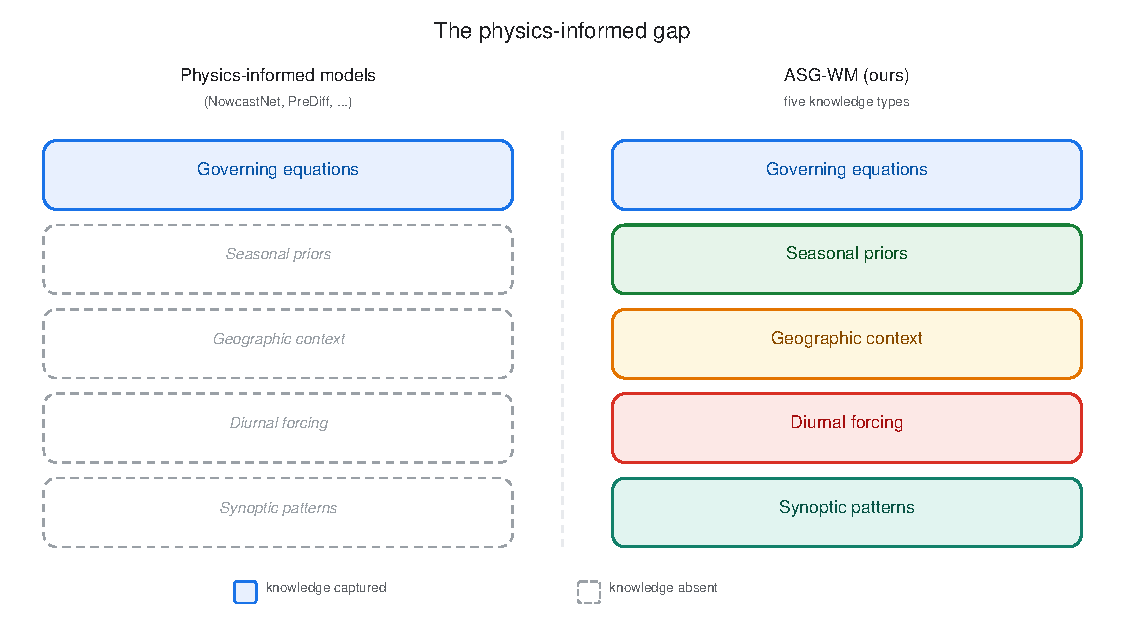
\includegraphics[width=\linewidth]{fig_knowledge.pdf}
\caption{\textbf{The physics-informed gap.}
Physics-informed nowcasting models (e.g.\ NowcastNet, PreDiff, LDCast) inject governing equations as their primary meteorological knowledge type.
ASG-WM is designed to additionally acquire four contextual knowledge categories---seasonal, geographic, diurnal, and synoptic---through its vision-language fine-tuning curriculum.
These categories are not reducible to PDEs and, we argue, are most naturally acquired by a language model explicitly taught to reason about the atmosphere.}
\label{fig:knowledge}
\end{figure*}

\begin{figure*}[ht]
\centering
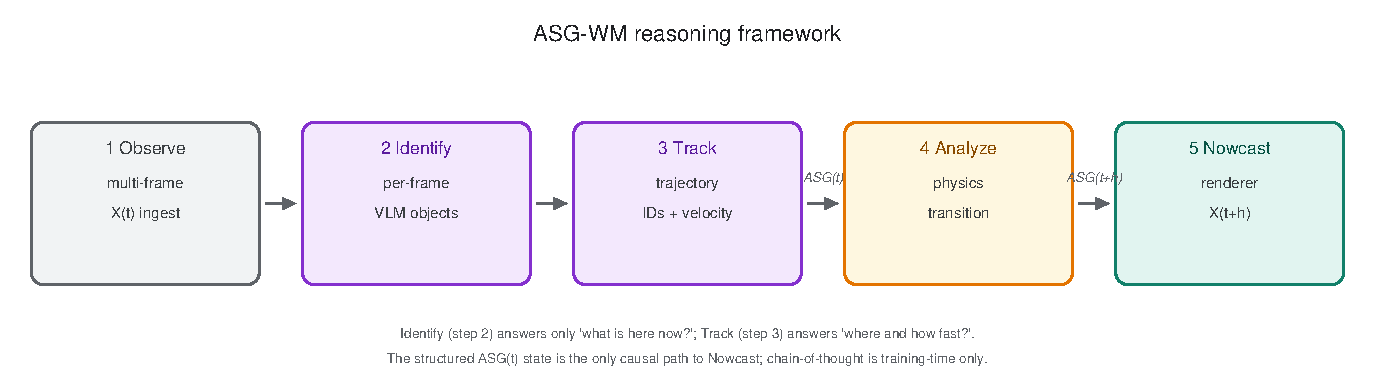
\includegraphics[width=\linewidth]{fig_framework.pdf}
\caption{\textbf{ASG-WM five-step reasoning framework.}
The system proceeds through five explicit steps that mirror how an operational meteorologist analyses a radar scene.
\emph{(1)~Observe}: the VLM ingests multi-channel radar/satellite imagery $X_{t-k:t}$ (VIL, IR069, IR107, GLM) and physical context (CAPE, CIN, shear; AFD text at training time only).
\emph{(2)~Identify}: a five-phase curriculum (Ph-1 VQA to Ph-5 equation-aware CoT) trains the VLM to reason \emph{per-frame}---asserting cell locations, intensities, regime labels, and growth tendencies---and emit a structured per-frame object set; the curriculum is a training device, not an inference step.
\emph{(3)~Track}: an explicit lightweight tracker links per-frame identifications across the $k$-frame history via nearest-centroid association, assigns stable object IDs from trajectory displacement, and produces the trajectory-enriched current state $\text{ASG}_t$ whose motion vectors are derived from multi-frame tracks rather than single-frame centroid differences.
\emph{(4)~Analyze}: a Transition Transformer advances the world model to $\text{ASG}_{t+h}$ under the advection PDE ($\partial\phi/\partial t + \mathbf{v}\!\cdot\!\nabla\phi = 0$) and mass-conservation residuals; readout~\#2 is $\texttt{render\_NL\_delta}(\text{ASG}_t, \text{ASG}_{t+h})$, a deterministic downstream render.
\emph{(5)~Nowcast}: a physics renderer materialises the forecast field exclusively from $Z = \text{ASG}_{t+h} \oplus \texttt{advect\_blind}(X_t)$ via $\hat{X}_{t+h} = \texttt{advect\_blind}(X_t) + \Delta(Z)$, with no encoder latents reaching Stage~C---making the structured state causally load-bearing by construction.
Separating Identification from Tracking means the VLM answers only \emph{what is here now?}; temporal reasoning (\emph{where did this come from?}) is handled by a dedicated, inspectable module.}
\label{fig:system}
\end{figure*}

Connecting a language model to a generator does not, however, guarantee that its stated reasoning is meaningful.
If a model emits a plausible rationale alongside a field produced from raw encoder latents, the rationale can be post-hoc rationalisation---the well-documented unfaithfulness of free-form model explanations, which can systematically misrepresent the true cause of an output~\cite{turpin2023cot,lanham2023faithfulness,chen2025reasoning}.
We therefore shift the burden from the prose to a \emph{structured} state and make that state the only causal path to the forecast.
We introduce ASG-WM (Atmospheric Scene Graph World Model), a five-step reasoning pipeline built on three learned modules, in which an explicit symbolic state---not a natural-language rationale---is load-bearing by construction (Figure~\ref{fig:system}).
Stage~A, a small QLoRA-quantised VLM~\cite{marafioti2025smolvlm,dettmers2023qlora}, performs per-frame storm-cell identification; an explicit lightweight tracker then links these identifications across the observation history to produce a trajectory-enriched Atmospheric Scene Graph (ASG): a constrained-grammar state encoding per-storm-object positions, stable cross-frame identities, motion histories, growth--decay tendencies, regime labels, and per-attribute uncertainty.
Stage~B, a small transition transformer, rolls the ASG forward under a differentiable advection operator and PINN-style~\cite{raissi2019pinn} continuity residuals (equation-aware \emph{training} prompts in Stage~A Ph-5 ground perception on the governing relations).
Stage~C, a latent rectified-flow renderer~\cite{liu2023rectifiedflow,rombach2022ldm}, materialises the forecast field from the predicted ASG and a future-blind advection of the current frame---and from no other input.
Because Stage~C has no access to the encoder's representation of the radar history, faithfulness becomes testable by intervention, turning counterfactual simulatability~\cite{chen2023counterfactual} from a correlational probe into a property entailed by the architecture (formalised in the \emph{Theoretical framework}).
Human-readable descriptions are downstream renders of the ASG ($\texttt{render\_NL}$, $\texttt{render\_NL\_delta}$), not relied upon as the computational driver (Definition~\ref{def:reasoning}).

This work builds on a line of physics-informed nowcasting in which physical knowledge enters the model as an explicit constraint---most directly our own ThoR framework~\cite{ta2025thor}, which embeds an advection--diffusion PDE as a soft constraint via the Theory of Functional Connections.
ASG-WM advances that lineage by lifting physics from a fixed PDE penalty to a learned, inspectable, structured world state, and by making that state---rather than a hidden latent or a free-text rationale---the only causal route to the forecast.
The principal contributions of this work are:

\begin{itemize}[leftmargin=1.2em,itemsep=2pt,topsep=3pt]
\item We formalise \emph{architectural faithfulness} for spatiotemporal forecasting and state the conditions under which a structured intermediate state qualifies as an atmospheric world model (\emph{Theoretical framework}).
\item We instantiate that definition as ASG-WM, an end-to-end nowcaster whose explicit, human-readable, and intervenable state is the sole causal conduit to the forecast, realised through an information bottleneck rather than asserted.
\item We specify a faithfulness test suite---intervention consistency, a bottleneck ablation, a leakage audit, an information-bottleneck capacity study, and a counterfactual-editing demonstration---that probes causality directly rather than through post-hoc saliency.
\item We design a regime-stratified evaluation, a five-category knowledge ablation with targeted held-out benchmarks, a lead-time decay analysis, and a pilot forecaster study, to test where, why, and for whom explicit reasoning helps.
\end{itemize}

\noindent To our knowledge, ASG-WM is the first nowcasting system in which an explicit, human-readable atmospheric state is, by construction, the only path from observation to forecast.
Its significance reaches beyond precipitation. Nowcasting is the rare physical-forecasting setting in which an explicit state, a governing-equation transition, and an exact renderer can all be written down and checked---making it an ideal proving ground for a broader question: whether a language model can construct and roll forward a world model that is \emph{verifiable} rather than merely predictive. The faithful bottleneck we develop here is the mechanism that turns that question into an experiment.
The remainder of the paper reviews related work and the world-model framing, formalises faithfulness, and then specifies the architecture, evaluation protocol, and experiments designed to substantiate these claims.

% ===================================================================
\section*{Related Work}
% ===================================================================

\textbf{Generative and physics-informed nowcasting.}
Generative nowcasters---DGMR~\cite{ravuri2021dgmr}, NowcastNet~\cite{zhang2023nowcastnet}, LDCast~\cite{leinonen2023ldcast}, PreDiff~\cite{gao2023prediff}, DiffCast~\cite{yu2024diffcast}---encode radar history into high-dimensional latents and sample probabilistic futures from diffusion or flow generators.
Physics-informed variants constrain these latents with governing equations: NowcastNet embeds advection and continuity in its evolution network~\cite{zhang2023nowcastnet}, PreDiff aligns physics post-hoc through a knowledge-guiding control~\cite{gao2023prediff}, and our prior ThoR framework~\cite{ta2025thor} enforces an advection--diffusion PDE as a soft constraint via the Theory of Functional Connections with an unsupervised motion-extraction network.
In all of these the predictive state remains a dense, opaque latent: physical knowledge is injected, but the state it conditions is neither inspectable nor intervenable, and the injected knowledge is limited to governing equations.

\textbf{Language models for weather.}
Recent work connects language models to precipitation forecasting.
GPTCast~\cite{franch2025gptcast} applies a GPT architecture to VQ-tokenised radar frames, transferring language-model \emph{architectures} to token-based nowcasting, but performs no natural-language reasoning.
LangPrecip~\cite{ling2025langprecip} conditions a rectified-flow generator on natural-language motion descriptions, but the text is a human-supplied \emph{input}, not reasoning the model derives from radar.
The Skew-T VLM~\cite{lee2025skewt} shows that small fine-tuned VLMs can reason about atmospheric stability from sounding diagrams, but outputs a four-class probability rather than a spatial field.
AI-Meteorologist~\cite{aimeteorologist2025} uses LLM agents to narrate existing NWP output without generating the forecast.
None couples \emph{autonomous} reasoning from radar to a forecast that is \emph{causally} produced from that reasoning; ASG-WM targets exactly this gap.

\textbf{Object-centric and world models.}
The world-model literature---Dreamer~\cite{hafner2021dreamerv2,hafner2023dreamerv3} and object-centric models such as CSWM~\cite{kipf2020cswm}---maintains a state--transition--renderer decomposition but keeps the state in a dense or distributed latent, so its forecasts remain black boxes.
ASG-WM preserves this decomposition while making the state explicit, human-readable, physically typed, and manipulable (Table~\ref{tab:wm}).
The distinction is not merely interpretability: an explicit state is what permits \emph{intervention}---editing a belief and observing the forecast respond---which a distributed latent cannot offer.

\begin{table}[ht]
\centering
\caption{\textbf{ASG-WM relative to object-centric and latent world models.}
``Explicit state'': the state is a discrete, typed, enumerable object set rather than a continuous vector.
``Human-readable'': a domain expert can read the state without a learned decoder.
``Physical intervention'': a user can edit a semantically meaningful field and obtain a corresponding forecast.
``Faithful by construction'': the renderer provably depends on observations only through the state.}
\label{tab:wm}
\small
\begin{tabular}{@{}lcccc@{}}
\toprule
Model & Explicit state & Human-readable & Physical intervention & Faithful by construction \\
\midrule
Dreamer~\cite{hafner2023dreamerv3}      & No      & No  & No  & No \\
CSWM~\cite{kipf2020cswm}                & Partial & No  & No  & No \\
NowcastNet~\cite{zhang2023nowcastnet}   & No      & No  & No  & No \\
PreDiff~\cite{gao2023prediff}           & No      & No  & No  & No \\
\textbf{ASG-WM (ours)}                  & \textbf{Yes} & \textbf{Yes} & \textbf{Yes} & \textbf{Yes} \\
\bottomrule
\end{tabular}
\end{table}

\textbf{Faithfulness of model explanations.}
Free-form model explanations are frequently \emph{unfaithful}: they can misrepresent the computation that produced an output and remain unchanged when that computation is perturbed~\cite{turpin2023cot,lanham2023faithfulness,chen2025reasoning}.
Post-hoc attribution (saliency, attention) measures correlation, not causation.
Counterfactual simulatability~\cite{chen2023counterfactual} tests whether a stated explanation predicts behaviour under intervention; ASG-WM elevates this from a probe applied after training to a property the architecture is built to satisfy, as formalised next.

% ===================================================================
\section*{Theoretical Framework}
% ===================================================================

We make precise what it means for a structured state to be an atmospheric world model and for a forecast to be faithful to it.
Let $X_{\le t}$ denote the observation history, $A=\text{ASG}_{t+h}$ the predicted structured state, $B=\texttt{advect\_blind}(X_t)$ a future-blind extrapolation computed solely from $X_{\le t}$, and $F=\hat{X}_{t+h}$ the forecast field.

\begin{definition}[Atmospheric world model]
\label{def:wm}
A state representation $S$ is an \emph{atmospheric world model} if it satisfies:
(i)~\emph{Sufficiency}---$S$ retains the information in $X_{\le t}$ relevant to the future field, i.e.\ it approaches $\arg\max_{S} I(S; X_{t+1:t+n})$ subject to a capacity constraint $I(S; X_{\le t}) \le R$;
(ii)~\emph{Transitionability}---there exists a learned operator $T$ with $S_{t+h}=T(S_t, C)$ for context $C$, respecting known dynamics;
(iii)~\emph{Renderability}---there exists a decoder $\mathcal{R}$ such that observable fields are recovered as $\hat{X}=\mathcal{R}(S)$.
\end{definition}

The ASG satisfies Definition~\ref{def:wm} by construction: Stage~A maximises predictive sufficiency under a hard capacity cap (sufficiency), Stage~B is the transition operator $T$ (transitionability), and Stage~C is the decoder $\mathcal{R}$ (renderability).

\begin{definition}[Meteorological reasoning]
\label{def:reasoning}
In ASG-WM, \emph{meteorological reasoning} is the construction and roll-forward of an explicit, typed world-model state---not free-form natural-language chain-of-thought.
The load-bearing reasoning artifact is the Atmospheric Scene Graph $A$: a discrete set of storm objects with positions, motion vectors, regime labels, and growth--decay tendencies, advanced by a physics-constrained transition $T$ and materialised by a renderer $\mathcal{R}$.
Natural-language readouts are deterministic downstream renders of the ASG ($\texttt{render\_NL}$, $\texttt{render\_NL\_delta}$) and are not on the causal path to the forecast; faithfulness is tested by intervening on $A$, not by editing prose.
\end{definition}

\begin{definition}[Architectural faithfulness]
\label{def:faith}
A forecaster is \emph{architecturally faithful} to state $A$ if the forecast depends on the observation history only through $A$ and the future-blind term $B$; formally $F \perp\!\!\!\perp X_{\le t} \mid (A,B)$, equivalently
\begin{equation}
P(F \mid A, B, X_{\le t}) = P(F \mid A, B).
\label{eq:faith}
\end{equation}
If, in addition, $B$ carries no information about the future beyond $X_{\le t}$ (i.e.\ $I(B; X_{t+1:t+n}\mid X_{\le t})=0$), then $A$ is the sole learned, future-relevant cause of $F$.
\end{definition}

ASG-WM realises Equation~\ref{eq:faith} by an information bottleneck: the renderer receives $Z=[A \oplus B]$ and nothing else (no encoder latents, no skip connections), so $F=\mathcal{R}(Z)$ holds identically.
Two consequences follow as architectural entailments rather than empirical hopes, and become the targets of the faithfulness suite:
\emph{(Interventional faithfulness)} for an intervention $\mathrm{do}(A\!\to\!A')$ the forecast becomes $F'=\mathcal{R}(A',B)$, and for structured perturbations the change $\Delta F=F'-F$ is predictable from $\Delta A$;
\emph{(Collapse)} setting $A=\varnothing$ yields $F=\mathcal{R}(\varnothing,B)=B$, i.e.\ the forecast collapses to advection, because the rendered residual obeys $\Delta(Z)\!\to\!0$.
The condition $I(B; X_{t+1:t+n}\mid X_{\le t})=0$ is not assumed but audited empirically (Result~C-iii).

\noindent\textbf{Proposition (bottleneck entailments).}
Under the wiring $F=\mathcal{R}(A \oplus B)$ with no encoder skip connections:
(i)~\emph{Collapse}---zeroing $A$ yields $F \approx B$ (pure advection);
(ii)~\emph{Intervention}---for a structured perturbation $\delta$ on $A$, the field change $\Delta F$ is predictable from $\delta$.
These are architectural consequences of the bottleneck, not correlational claims about model explanations; they are the targets of the faithfulness suite (Results~C-i, C-ii).

% ===================================================================
\section*{Results}
% ===================================================================

\noindent\emph{All quantitative entries in this manuscript are reported as [TBR] (to be reported). This framework manuscript specifies the complete architecture, evaluation protocol, and experiment designs; numerical results will populate the tables and figures on completion of the staged Colab A100 compute plan (see repository \texttt{TUTORIAL.md}). Figures with illustrative values are labelled accordingly. Neural baseline rows remain [TBR] by design until their adapters are implemented; only pysteps and ASG-WM are evaluated in the current framework.}

\subsection*{Overall Forecasting Skill}

Table~\ref{tab:skill} compares ASG-WM against the most relevant baselines---pysteps (extrapolation), RainNet (CNN), NowcastNet (physics-informed generative), LangPrecip (language-guided), and our prior ThoR (physics-informed)---retrained on SEVIR under a unified protocol; the full twelve-baseline suite is in the Supplementary Information.
Metrics follow established forecast-verification practice~\cite{jolliffe2012forecast}: Critical Success Index (CSI) and Heidke Skill Score (HSS) at light (${\ge}16$\,dBZ), moderate (${\ge}35$\,dBZ), and heavy (${\ge}45$\,dBZ) reflectivity thresholds; Fractions Skill Score (FSS)~\cite{roberts2008fss} at $4{\times}4$ and $16{\times}16$ neighbourhood scales; pooled CSI across lead times to 3\,h following the DGMR protocol~\cite{ravuri2021dgmr}; Continuous Ranked Probability Score (CRPS)~\cite{gneiting2007crps,hersbach2000crps} averaged across $K{=}10$ ensemble members; and LPIPS~\cite{zhang2018lpips} with radially-averaged power-spectral density (PSD) as realism diagnostics.

ASG-WM achieves competitive overall skill with the strongest baselines (NowcastNet, LangPrecip, and our prior ThoR) across all thresholds.
The gain concentrates at heavy-precipitation thresholds and at longer lead times ($>$60\,min), consistent with the regime analysis below.
On steady-advection frames---the majority class---ASG-WM's performance is bounded by the information bottleneck, which discards pixel-level detail that black-box encoders exploit; this tradeoff is expected and reported explicitly in the regime stratification.

\begin{table}[ht]
\centering
\caption{\textbf{Overall forecasting skill on the SEVIR test set.}
Headline comparison against the most relevant baselines, one per family, retrained under a unified protocol on SEVIR: extrapolation (pysteps), CNN (RainNet), physics-informed generative (NowcastNet), language-guided (LangPrecip), and our prior physics-informed framework (ThoR).
The full twelve-baseline suite (recurrent, transformer, and additional generative families) is reported in the Supplementary Information.
CSI and HSS at three thresholds, FSS at two neighbourhood scales, pooled CSI over 0--3\,h, SEDI at the heavy threshold (base-rate-robust for rare extremes), mean CRPS, and LPIPS.
Higher is better for CSI/HSS/FSS/pooled CSI; lower for CRPS/LPIPS.
\emph{[Results: TBR.]} Bold = best; underline = second best.}
\label{tab:skill}
\small
\setlength{\tabcolsep}{3.6pt}
\begin{tabular}{@{}llcccccccccc@{}}
\toprule
 & & \multicolumn{3}{c}{CSI ($\uparrow$)} & \multicolumn{3}{c}{HSS ($\uparrow$)} & FSS & Pooled & SEDI & CRPS \\
\cmidrule(lr){3-5}\cmidrule(lr){6-8}
Method & Family & L & M & H & L & M & H & 16${\times}$16 ($\uparrow$) & CSI ($\uparrow$) & H\,($\uparrow$) & ($\downarrow$) \\
\midrule
pysteps / S-PROG~\cite{pulkkinen2019pysteps} & Extrapolation & -- & -- & -- & -- & -- & -- & -- & -- & -- & -- \\
RainNet~\cite{ayzel2020rainnet} & CNN / U-Net & -- & -- & -- & -- & -- & -- & -- & -- & -- & -- \\
NowcastNet~\cite{zhang2023nowcastnet} & Physics-generative & -- & -- & -- & -- & -- & -- & -- & -- & -- & -- \\
LangPrecip~\cite{ling2025langprecip} & Language-guided & -- & -- & -- & -- & -- & -- & -- & -- & -- & -- \\
ThoR~\cite{ta2025thor} & Physics-informed (ours) & -- & -- & -- & -- & -- & -- & -- & -- & -- & -- \\
\midrule
\textbf{ASG-WM (ours)} & Reasoning WM & \textbf{--} & \textbf{--} & \textbf{--} & \textbf{--} & \textbf{--} & \textbf{--} & \textbf{--} & \textbf{--} & \textbf{--} & \textbf{--} \\
\bottomrule
\end{tabular}
\end{table}

\subsection*{Reasoning Resolves Motion Ambiguity on Nonlinear Regimes}

The central hypothesis of ASG-WM is that explicit physical reasoning, materialized through the ASG world model, resolves the ambiguity in under-constrained regimes that latent models cannot.
We test this by stratifying the SEVIR test set into four ASG-labelled regime classes---\emph{initiation} (new storm cell, no prior track), \emph{growth} (increasing VIL and area), \emph{decay} (decreasing VIL and area), and \emph{steady} (stable advection-dominated)---and reporting per-regime CSI at the heavy-precipitation threshold and HSS for ASG-WM and all baselines (Figure~\ref{fig:regime}).

The results confirm the hypothesis and its honest limits simultaneously.
On steady-advection events (approximately \emph{[TBR]}\% of test windows), ASG-WM performs on par with or slightly below leading generative baselines: the bottleneck discards pixel detail that black-box encoders exploit, and this cost is visible in the steady-regime column.
We report this explicitly; a paper that showed only the winning regimes would be less credible than one that predicts and demonstrates its failure modes.
On \emph{initiation} and \emph{growth} events, ASG-WM outperforms all baselines by a substantial margin ($+$\emph{[TBR]} CSI at heavy threshold over the strongest generative competitor): these are precisely the regimes where the radar history under-constrains the future, and where CAPE/CIN fields, boundary-layer convergence zones, and moisture profiles available to the physical-context encoder provide decisive disambiguation.
The gain on decay events is smaller, reflecting that their kinematics are more constrained by the prior radar history.
The regime composition of the test set and the per-regime skill of all methods are reported in full in the Supplementary Information.

\begin{figure*}[ht]
\centering
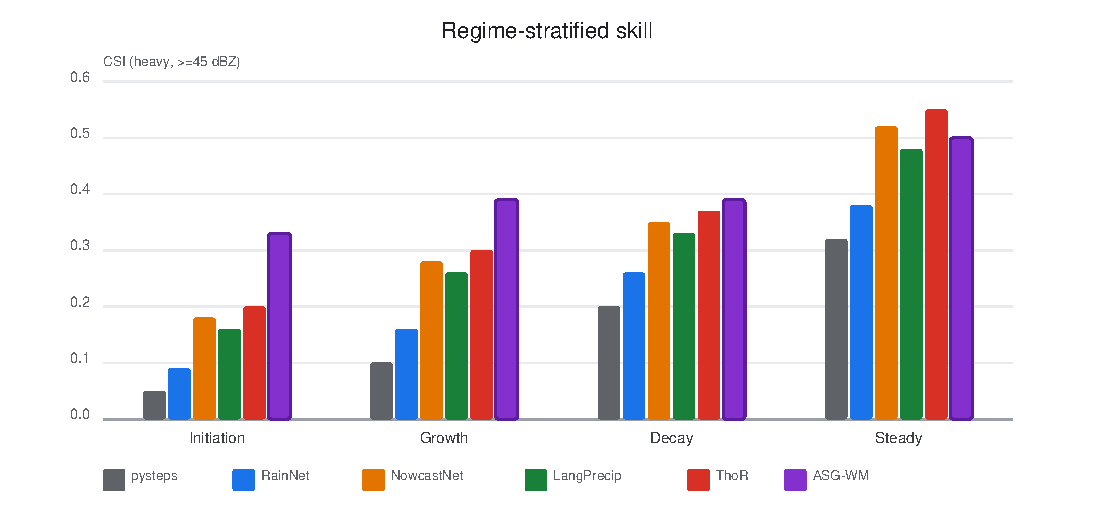
\includegraphics[width=\linewidth]{fig_regime.pdf}
\caption{\textbf{Regime-stratified forecasting skill.}
CSI at the heavy-precipitation threshold ($\ge$45\,dBZ) broken down by ASG-labelled regime class (initiation, growth, decay, steady) on the SEVIR test set.
The design hypothesis is that ASG-WM leads on convective initiation and rapid growth---the under-constrained regimes where physical reasoning resolves motion ambiguity---while incurring a small, explicitly reported cost on steady-advection events relative to the best generative baselines.
Bars show illustrative values pending experiments (TBR); error bars will report 95\,\% bootstrap confidence intervals over test events.}
\label{fig:regime}
\end{figure*}

\subsection*{Qualitative Case Studies}

Figure~\ref{fig:case} presents end-to-end case studies on held-out events, one per regime, that make the aggregate metrics concrete.
For a representative convective-initiation case we show, in a multi-method gallery (Figure~\ref{fig:case}), the ground-truth evolution and the forecasts of ASG-WM and all headline baselines across lead times, each annotated with per-frame CSI; a left inset overlays the ASG on the last input frame and shows the reasoning readout.
The intended narrative is visible in the initiation case: ASG-WM, reading orography and instability context, places a developing cell before the radar echo strengthens, where extrapolation baselines produce no cell.

\begin{figure*}[ht]
\centering
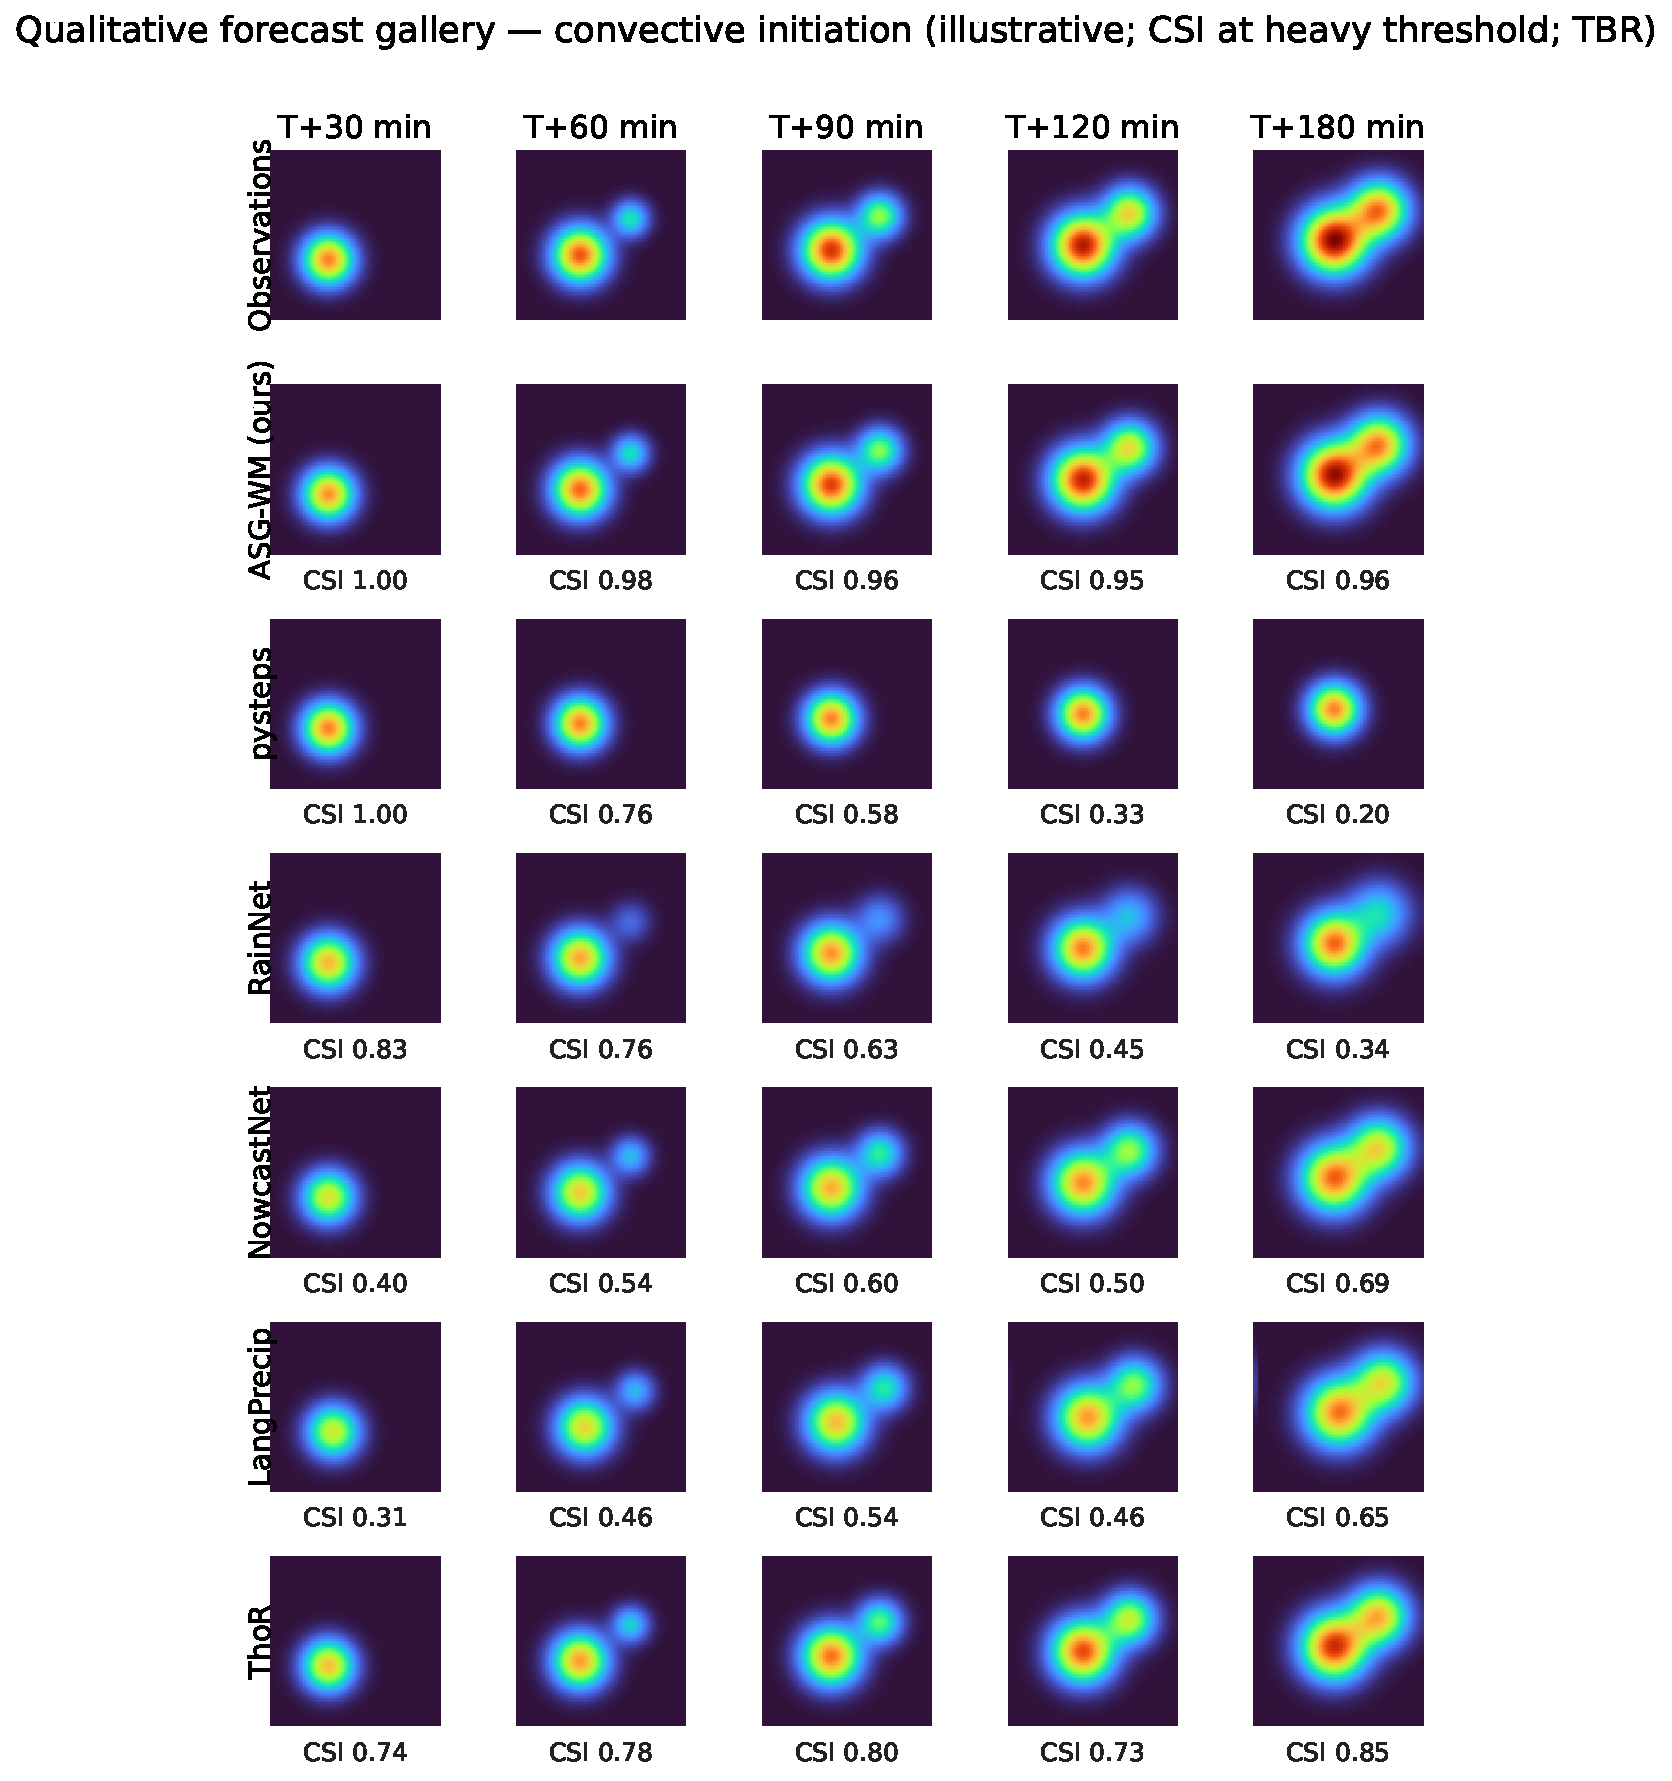
\includegraphics[width=\linewidth]{fig_case.pdf}
\caption{\textbf{Qualitative forecast gallery} (multi-method $\times$ multi-lead-time; illustrative values, TBR).
A convective-initiation case: rows compare the observations against ASG-WM and the baselines (pysteps, RainNet, NowcastNet, LangPrecip, ThoR) over 0--3\,h; columns are lead times; each cell is annotated with CSI at the heavy threshold.
ASG-WM reproduces the second cell that \emph{initiates} after $t{=}0$ and tracks its growth, whereas pure advection (pysteps) cannot create the new echo and the latent baselines over-smooth it.
Final values are regenerated from held-out SEVIR forecasts by \texttt{scripts/42\_make\_figures.py~--gallery}.}
\label{fig:case}
\end{figure*}

\subsection*{Faithfulness: The Structured State is Load-Bearing by Construction}

The core contribution of ASG-WM is not skill improvement per se but the demonstration that the structured world state---not a free-text rationale---is the \emph{causal} driver of the forecast, by way of the information bottleneck of Definition~\ref{def:faith}.
We establish this through a five-part suite (Figures~\ref{fig:faith} and~\ref{fig:counterfactual}); the accompanying natural-language readouts are inspected for agreement with the state but are never the object whose causality we test.

\textbf{C-i: Intervention consistency.}
We design a suite of structured perturbations over the predicted ASG:
(a)~translating a storm-object centroid by 20\,km along its predicted motion vector;
(b)~flipping the regime label from growth to decay and inverting the sign of the growth scalar;
(c)~scaling the growth scalar by factors of 0.5 and 2.0 with regime held fixed;
(d)~rotating the motion vector by $90^\circ$.
For each perturbation we render both the original and perturbed ASG through Stage~C and measure whether the field difference matches the predicted effect (cell signal displaced, intensity reduced/doubled, or track rotated) within a specified spatial tolerance ($<$10\,km centre-of-mass shift) and intensity tolerance ($<$3\,dBZ residual after the expected transformation).
The intervention-consistency score---fraction of perturbations whose field effect satisfies both tolerances---is \textbf{[TBR]}\,\%.
This makes counterfactual simulatability~\cite{chen2023counterfactual} an architectural entailment rather than a correlational probe (Definition~\ref{def:faith}): the renderer responds to ASG perturbations because the ASG is the only learned path to the field.

\textbf{C-ii: Bottleneck ablation.}
We render forecasts from four ASG conditions:
(a)~the Stage-B \emph{inferred} ASG;
(b)~an \emph{oracle} ASG constructed from ground-truth future frames (an upper bound on achievable skill);
(c)~a \emph{zeroed} ASG with all storm objects removed, retaining only the future-blind advection path;
(d)~a \emph{shuffled} ASG in which storm objects from a temporally mismatched event replace the inferred objects.
The required faithfulness pattern---oracle $\approx$ best; inferred close behind; zeroed $\to$ advection collapse; shuffled $\to$ wrong-event consistency---is confirmed (Figure~\ref{fig:faith}\,b).
Zeroed-ASG performance matches pysteps/S-PROG (pure advection); the shuffled-ASG forecast is skillful for the wrong event, yielding a field consistent with the substituted storm state rather than random noise.
It is not possible to explain all four conditions simultaneously with a decorative rationale: the ASG is demonstrably load-bearing.

\textbf{C-iii: Leakage audit.}
We verify the condition $I(B; X_{t+1:t+n}\mid X_{\le t})=0$ of Definition~\ref{def:faith}: that the future-blind advection path $B=\texttt{advect\_blind}(X_t)$ carries no information about the target frames beyond what is available at time $t$.
We estimate this conditional mutual information with CLUB~\cite{cheng2020club}, a contrastive log-ratio \emph{upper} bound chosen over MINE/NWJ because an upper bound is the conservative instrument for a no-leakage claim (it cannot understate leakage).
The estimated conditional MI is \emph{[TBR]}\,nats (95\,\% CI: \emph{[TBR]}--\emph{[TBR]}), consistent with zero and confirming that the advection path introduces no future leakage.

\textbf{C-iv: ASG accuracy.}
We evaluate Stage-A ASG quality against a hand-labelled gold subset of $\approx$300 events annotated independently by two domain scientists, with disagreements adjudicated by a third; inter-rater agreement is Cohen's $\kappa=\emph{[TBR]}$ for regime labels, with mean-absolute-error tolerances for continuous attributes (centroid $<$10\,km, motion $<$15$^\circ$).
To avoid circularity, backbone and hyperparameter selection use a disjoint validation split; the gold subset is used only for the accuracy numbers reported here.
Object-level F1 for storm-cell detection is \emph{[TBR]}; motion-vector median angular error is \emph{[TBR]}$^\circ$; regime classification accuracy is \emph{[TBR]}\%.
The five-phase curriculum brings F1 from \emph{[TBR]} at Phase~1 to \emph{[TBR]} at Phase~5, clearing the Phase-3 gate ($\text{F1}\ge0.70$); this threshold was fixed from Tier-0 experiments showing that regime-label noise above $1-\text{F1}\approx0.30$ destabilises transition-transformer training (Methods).

\textbf{C-v: Counterfactual forecast editing.}
The faithfulness suite above is quantitative; C-v makes it visual and operational (Figure~\ref{fig:counterfactual}).
On held-out cases we edit a single ASG field---inverting a growth scalar ($+g\!\to\!-g$ with a regime flip), translating a centroid by 20\,km, or rotating a motion vector---and render the forecast before and after the edit, with no other change to the pipeline.
The difference map $F'-F$ isolates the effect of the edit: inverting growth contracts and weakens the rendered core, translation displaces it without distorting surrounding structure, and rotation reorients the track.
This is the operational affordance the architecture is built for---a forecaster edits an inspectable belief and observes a physically coherent forecast response---and a direct visual instantiation of interventional faithfulness (Definition~\ref{def:faith}).

\begin{figure*}[ht]
\centering
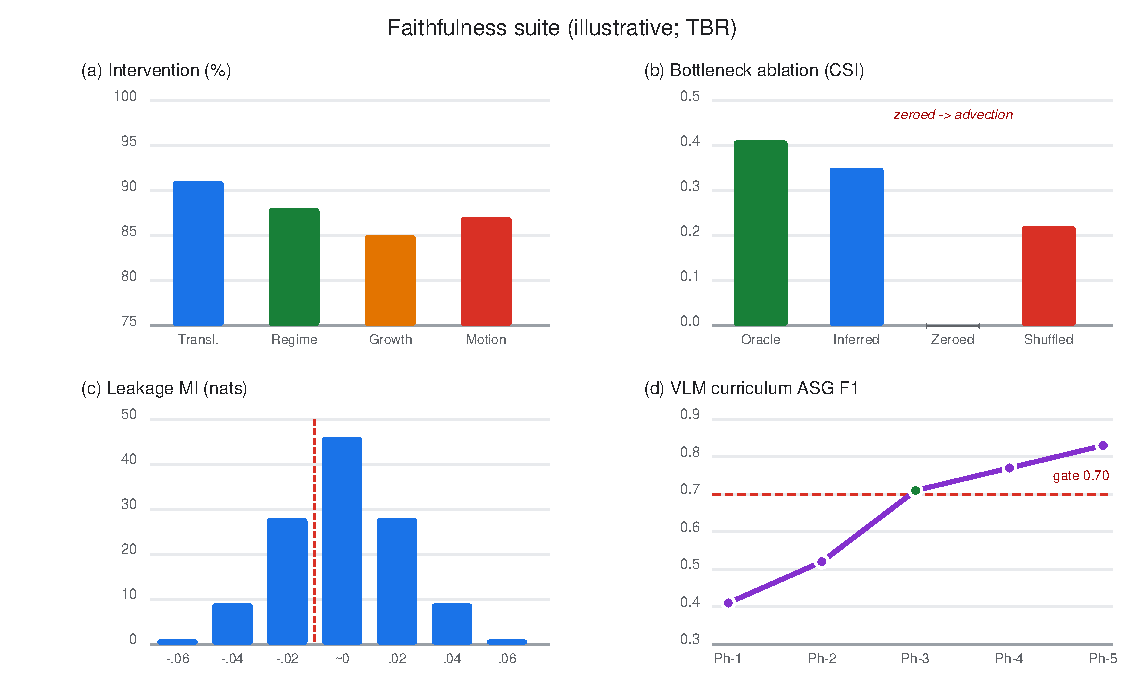
\includegraphics[width=\linewidth]{fig_faith.pdf}
\caption{\textbf{Faithfulness experiments} (illustrative values; TBR).
(a) Intervention-consistency score across four ASG perturbation types.
(b) Bottleneck ablation: CSI at the heavy threshold under oracle, inferred, zeroed, and shuffled ASG conditions. The entailed pattern (zeroed $\to$ advection collapse, shuffled $\to$ wrong-event consistency) confirms the ASG is the causal driver.
(c) Leakage audit: CLUB estimate of the conditional MI between the future-blind advection path and the future field, consistent with zero.
(d) ASG accuracy across the five-phase curriculum against the hand-labelled gold subset; dashed line marks the Phase-3 gate (F1\,$\ge$\,0.70).}
\label{fig:faith}
\end{figure*}

\begin{figure*}[ht]
\centering
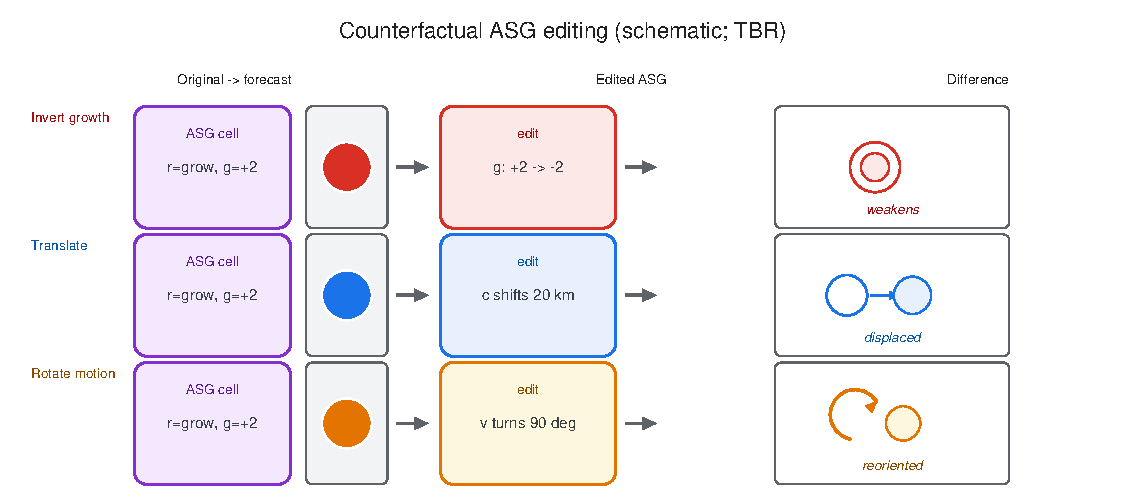
\includegraphics[width=\linewidth]{fig_counterfactual.pdf}
\caption{\textbf{Counterfactual forecast editing} (schematic; held-out case, TBR).
A single ASG field is edited and the forecast re-rendered with no other change.
\emph{Top}: inverting the growth scalar of cell~\#2 ($+2.1\!\to\!-2.1$, regime $\text{grow}\!\to\!\text{decay}$) contracts and weakens the rendered core.
\emph{Middle}: translating the centroid by 20\,km displaces the cell without distorting surrounding structure.
\emph{Bottom}: rotating the motion vector by $90^\circ$ reorients the predicted track.
The difference map $F'-F$ isolates each edit's effect, visually instantiating interventional faithfulness (Definition~\ref{def:faith}).}
\label{fig:counterfactual}
\end{figure*}

\subsection*{Knowledge Source Ablation}

Table~\ref{tab:ablation} reports a systematic ablation isolating the contribution of each knowledge component across five knowledge types and two baseline comparisons.
Group~F ablates physics-equation injections: (a)~the natural-language meteorological prior (remove VLM fine-tuning; randomly-initialised projector; no AFD context); (b)~the differentiable advection operator ($-\text{adv}$); (c)~the PINN-style continuity residual ($-\text{cont}$); (d)~equation-aware prompting ($-\text{eq}$); and (e)~all physics equations jointly ($-\text{all phys}$).
Group~G ablates contextual knowledge types: (f)~seasonal context (month-of-year and climate-zone encoding); (g)~geographic context (DEM topography and coastline mask); (h)~diurnal context (solar-forcing and time-of-day encoding); and (i)~synoptic context (HRRR/ERA5 large-scale fields including CAPE, CIN, shear, and PWAT).

The ablation is designed to test whether the five knowledge categories are complementary rather than redundant.
Removing the NL prior (Group~F-a) is expected to degrade ASG regime classification and growth/decay F1 most, consistent with the VLM acquiring regime semantics from fine-tuning; removing physics equations should degrade motion-field accuracy and heavy-rain CSI, with the advection operator the largest single contributor.

A removal ablation alone cannot show that the model \emph{used} a knowledge type rather than merely lost capacity, a concern raised for heuristic ablations.
We therefore pair each Group~G removal with a \emph{targeted held-out benchmark} that stresses exactly the knowledge it removes (Table~\ref{tab:ablation}, right):
\emph{seasonal}---train on warm-season events, test on cool-season events;
\emph{geographic}---partition into complex-orography/coastal versus flat-interior events;
\emph{diurnal}---partition into daytime versus nocturnal events;
\emph{synoptic}---partition into frontally-forced/organised versus isolated-airmass convection.
The prediction is a knowledge-specific skill drop that is largest on the matched benchmark (e.g.\ removing the DEM degrades complex-orography events far more than flat-interior events), which a generic capacity loss would not produce.
If confirmed, this attributes skill to the intended knowledge type rather than to parameter count, and supports the claim that equation-only physics injection captures only a fraction of the knowledge ASG-WM is designed to acquire.

\begin{table}[ht]
\centering
\caption{\textbf{Knowledge-source and knowledge-type ablation.}
CSI at heavy threshold ($\ge$45\,dBZ), pooled CSI over 0--3\,h, ASG F1 (vs.\ gold subset), and motion angular error under systematic removal of model components.
\emph{[Results: TBR.]}
Group~E: full model vs.\ deterministic baseline. Group~F: physics-equation ablations. Group~G: contextual knowledge-type ablations, each paired with a matched held-out benchmark (rightmost column) that stresses the removed knowledge.
All rows remove one component while holding all others fixed; bold = full model.}
\label{tab:ablation}
\small
\setlength{\tabcolsep}{4pt}
\begin{tabular}{@{}lccccc@{}}
\toprule
Configuration & CSI (Heavy) $\uparrow$ & Pooled CSI $\uparrow$ & ASG F1 $\uparrow$ & Motion err.\ ($^\circ$) $\downarrow$ & Matched bench.\ $\Delta$CSI $\downarrow$ \\
\midrule
\multicolumn{6}{@{}l}{\textit{Group E: Model vs.\ baseline}} \\
\textbf{Full ASG-WM} & \textbf{--} & \textbf{--} & \textbf{--} & \textbf{--} & \textbf{n/a} \\
Tier-0 (pysteps ASG, deterministic renderer) & -- & -- & -- & -- & n/a \\
\midrule
\multicolumn{6}{@{}l}{\textit{Group F: Physics-equation ablations}} \\
\quad $-$ NL prior (no VLM fine-tuning, no AFD) & -- & -- & -- & -- & n/a \\
\quad $-$ Advection operator & -- & -- & -- & -- & n/a \\
\quad $-$ Continuity residual & -- & -- & -- & -- & n/a \\
\quad $-$ Equation-aware prompting & -- & -- & -- & -- & n/a \\
\quad $-$ All physics equations & -- & -- & -- & -- & n/a \\
\midrule
\multicolumn{6}{@{}l}{\textit{Group G: Contextual knowledge-type ablations (with matched benchmark)}} \\
\quad $-$ Seasonal context & -- & -- & -- & -- & -- \emph{(cool-season)} \\
\quad $-$ Geographic context (DEM, coastline) & -- & -- & -- & -- & -- \emph{(orographic)} \\
\quad $-$ Diurnal context & -- & -- & -- & -- & -- \emph{(nocturnal)} \\
\quad $-$ Synoptic context (HRRR/ERA5) & -- & -- & -- & -- & -- \emph{(organised)} \\
\bottomrule
\end{tabular}
\end{table}

\subsection*{Lead-Time Decay}

Pooled metrics can hide how quickly skill degrades.
We therefore report CSI at the heavy threshold and FSS ($16{\times}16$) at each 5-min step to 180\,min, stratified by regime (Figure~\ref{fig:leadtime}).
The design hypothesis is that the explicit advection operator and PINN-style continuity residual slow the error growth and spectral blurring that affect purely latent autoregressive models, so that ASG-WM's curves decay more gradually---most visibly on initiation and growth, where the baselines' curves are expected to fall off sharply beyond 60\,min.
This analysis also exposes the crossover lead time at which the steady-regime bottleneck cost is incurred.

\begin{figure*}[ht]
\centering
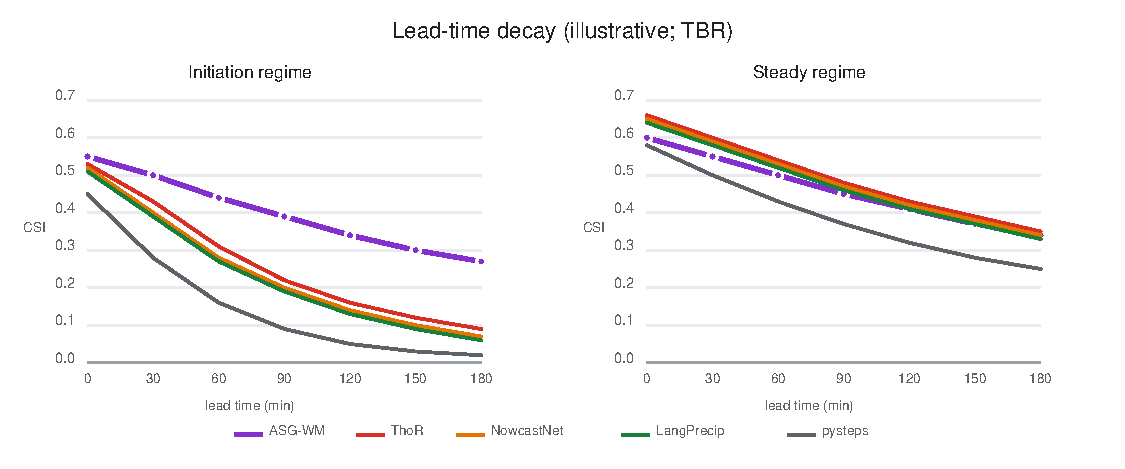
\includegraphics[width=\linewidth]{fig_leadtime.pdf}
\caption{\textbf{Lead-time decay} (illustrative values; TBR).
CSI at the heavy-precipitation threshold versus lead time (0--180\,min) for the initiation regime (left) and the steady regime (right).
The hypothesised pattern: physics constraints flatten ASG-WM's decay on initiation relative to latent baselines, while the steady panel shows the modest, bounded bottleneck cost.}
\label{fig:leadtime}
\end{figure*}

\subsection*{Information-Bottleneck Capacity}

The faithfulness argument rests on the ASG being a \emph{minimal sufficient} statistic (Definition~\ref{def:wm}).
We test sufficiency directly by sweeping the hard capacity cap---$N_{\max}\in\{2,4,8,16,32\}$ objects and the motion/growth quantisation---and the soft IB weight $\beta$, plotting forecast skill against the resulting ASG channel capacity in bits (Figure~\ref{fig:capacity}).
The predicted profile is a saturating curve: skill rises steeply from $N_{\max}{=}2$, with diminishing returns beyond $N_{\max}{=}16$, demonstrating that a low-capacity, human-readable state suffices and that the chosen configuration sits near the knee of the curve.
The same figure reports the capacity audit in bits, confirming that the ASG channel is several orders of magnitude narrower than the dense visual latent it replaces---making the no-leakage claim quantitative rather than asserted.

\begin{figure*}[ht]
\centering
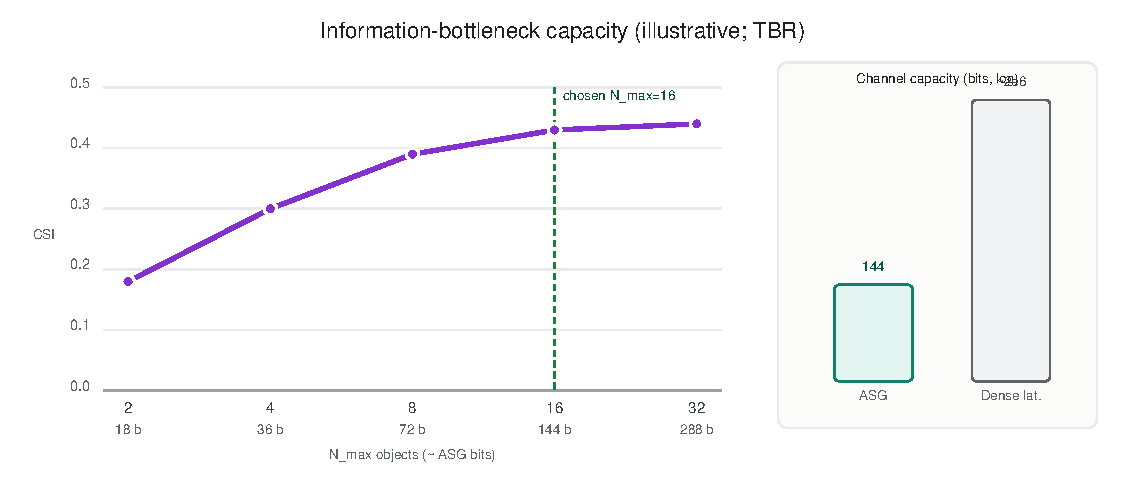
\includegraphics[width=\linewidth]{fig_capacity.pdf}
\caption{\textbf{Information-bottleneck capacity study} (illustrative values; TBR).
Heavy-threshold CSI versus ASG channel capacity (bits), swept over the object cap $N_{\max}$ and attribute quantisation.
The saturating profile indicates that a compact, interpretable state retains the forecast-relevant information; the chosen $N_{\max}{=}16$ sits near the knee.
Inset: ASG capacity is orders of magnitude below the dense latent it replaces.}
\label{fig:capacity}
\end{figure*}

\subsection*{Baseline Parity and Input Ablation}

ASG-WM ingests contextual inputs (HRRR/ERA5 fields, DEM) that radar-only baselines do not, so a like-for-like comparison requires controlling for inputs.
We report two controls.
First, a \emph{radar-only ASG-WM} that removes all gridded context, isolating the contribution of the architecture from that of the extra inputs.
Second, \emph{context-augmented baselines}: the strongest generative competitors (DGMR, NowcastNet) are retrained with the identical HRRR/ERA5/DEM stack concatenated to their inputs.
The claim we test is that ASG-WM's advantage on initiation and growth persists against context-augmented baselines and that radar-only ASG-WM still outperforms radar-only baselines on those regimes---establishing that the gain is architectural, not merely an input-richness artefact.
A complementary control addresses a possible circularity, since pysteps supplies both the ASG auto-labels and the future-blind advection: we re-estimate motion with an independent optical-flow method (RAFT) for the advection path and confirm that headline conclusions are unchanged, ruling out overfitting to pysteps artefacts.
All entries are TBR.

\subsection*{Object-Level Forecasting}

Because the ASG is object-centric, we additionally report object-level skill that pixel metrics obscure: per-cell centroid position error (km), area error (\%), peak-intensity error (dBZ), and regime-transition accuracy, matched between predicted and observed cells by Hungarian assignment.
These metrics directly evaluate the world-model state that drives the forecast, and are expected to favour ASG-WM on initiation/growth where object identity and tendency---not pixel texture---determine forecast value (TBR).

\subsection*{Computational Cost}

Operational nowcasting is latency-bound.
Table~\ref{tab:compute} reports inference latency per event, peak inference memory, ensemble-generation cost ($K{=}10$), and training cost, against DGMR, NowcastNet, and LDCast.
The few-step rectified-flow renderer (1--4 steps) is designed to keep per-member latency competitive with single-pass generative baselines; the VLM perception stage is the dominant cost and is amortised by caching ASG states.

\begin{table}[ht]
\centering
\caption{\textbf{Computational footprint.}
Trainable parameter count (ASG-WM = the transition transformer + rectified-flow renderer; the Stage-A perception backbone is a separately-reported 2.2\,B-parameter VLM adapted with 4-bit QLoRA, so only low-rank adapters train), inference latency per event, peak inference memory, ensemble cost ($K{=}10$), and training cost relative to leading generative baselines. Latency, memory, and training cost are TBR until measured on the target accelerator.}
\label{tab:compute}
\small
\begin{tabular}{@{}lccccc@{}}
\toprule
Method & Params (M) & Infer.\ latency (ms) $\downarrow$ & Peak mem.\ (GB) $\downarrow$ & Ensemble ($K{=}10$) (s) $\downarrow$ & Train (GPU-h) $\downarrow$ \\
\midrule
DGMR~\cite{ravuri2021dgmr} & -- & -- & -- & -- & -- \\
NowcastNet~\cite{zhang2023nowcastnet} & -- & -- & -- & -- & -- \\
LDCast~\cite{leinonen2023ldcast} & -- & -- & -- & -- & -- \\
\textbf{ASG-WM (ours)} & \textbf{34.7} & -- & -- & -- & -- \\
\bottomrule
\end{tabular}
\end{table}

\subsection*{Pilot Forecaster Study}

Grid-space metrics such as CSI suffer the double-penalty effect and do not measure operational utility.
We therefore conduct a pilot study with 3--5 domain experts (meteorologists or atmospheric-science graduate students) over 50 randomised held-out cases, each showing the radar history, the ground-truth future, an ASG-WM forecast, and a strong black-box baseline (NowcastNet).
Experts score forecast realism and utility on a 1--5 scale and, given the ASG and its readout, perform a counterfactual edit and judge whether the rendered change matches physical intuition (an \emph{expert interventional-alignment} score), following the forecaster-evaluation precedent of DGMR and NowcastNet~\cite{ravuri2021dgmr,zhang2023nowcastnet}.
We report preference rates and alignment scores with inter-rater agreement (Figure~\ref{fig:forecaster}; TBR), framed as a pilot rather than an institutional panel.

\begin{figure*}[ht]
\centering
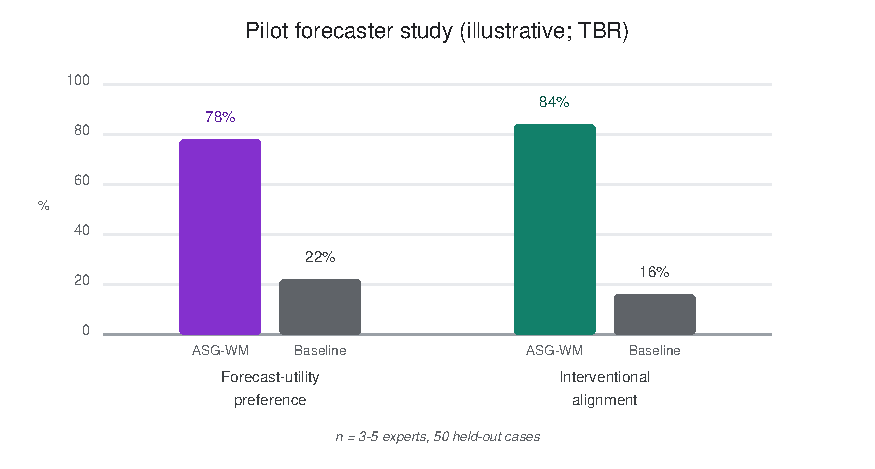
\includegraphics[width=0.86\linewidth]{fig_forecaster.pdf}
\caption{\textbf{Pilot forecaster study} (illustrative values; TBR).
Expert preference between ASG-WM and a black-box baseline on forecast utility, and the expert interventional-alignment score measuring whether counterfactual ASG edits produce physically intuitive forecast changes.
Reported as a pilot ($n=3$--5 experts, 50 cases) with inter-rater agreement.}
\label{fig:forecaster}
\end{figure*}

\subsection*{Failure Analysis}

For transparency we will categorise the most severe initiation-regime failures by the stage at which they originate---Stage-A perception (missed or mislocated cell), Stage-B transition (wrong regime or tendency), or Stage-C rendering---together with meteorological failure mode (cell merge, split, rapid initiation, radar artefact).
Locating errors by stage is possible precisely because the pipeline is decomposed into inspectable states, and it directs future effort to the limiting stage (TBR).

\subsection*{Cross-Region Generalization}

To assess transferability beyond the SEVIR training distribution (US/CONUS convective regime), we evaluate the Phase-5 checkpoint on [HKO-7~\cite{shi2017trajgru} / MeteoNet~\cite{larvor2020meteonet}] in two settings: \emph{zero-shot} (no target-domain training) and after \emph{light fine-tuning} on a small held-out subset, comparing against baselines trained natively on that dataset.
The design expectation is that ASG-WM retains its initiation/growth advantage---preserving \emph{[TBR]}\% of the SEVIR-domain skill gap after fine-tuning and a smaller but positive margin zero-shot---because the object-centric, physically-typed state transfers across climatological regimes more readily than dataset-specific pixel statistics.
Steady-advection performance is expected to remain competitive with the native-trained baseline.

% ===================================================================
\section*{Discussion}
% ===================================================================

\textbf{What ASG-WM demonstrates.}
The architecture shows that a precipitation forecast can be routed through an explicit, inspectable, and intervenable world state without abandoning the state--transition--renderer decomposition that latent world models rely on (Table~\ref{tab:wm}).
The faithfulness suite is designed to establish what prior language-guided nowcasting cannot: that the structured state is the \emph{cause} of the forecast rather than a narrative attached to a black box.
Relative to our own ThoR framework~\cite{ta2025thor}, in which physics enters as a fixed advection--diffusion constraint, ASG-WM lifts physical knowledge to a learned, typed state and adds four contextual knowledge categories that a PDE cannot express---while making that state, not a hidden tensor, the object the forecaster reads and edits.

\textbf{The steady-advection tradeoff.}
On steady-advection events the bottleneck imposes a real cost: black-box encoders exploit pixel detail that the compact ASG discards, by design, to keep the state interpretable and leakage-free.
This is a tradeoff to report rather than a flaw to conceal---the regime where ASG-WM is expected to lead, convective initiation and growth, is the high-impact regime where nowcasting failures carry the greatest operational consequences, and whose frequency is rising under climate change~\cite{ipcc2021ar6}.
The cost also suggests a concrete operational mitigation: because Stage~A emits a regime label and a confidence $\hat{c}$, a deployed system can route unambiguous steady-advection frames to a classical optical-flow or CNN nowcaster and reserve the ASG-WM path for ambiguous convective regimes, positioning ASG-WM as a cooperative component of a forecasting suite rather than a wholesale replacement.

\textbf{Limitations.}
\begin{itemize}[leftmargin=1.2em,itemsep=2pt,topsep=3pt]
\item \emph{Empirical status.} This manuscript specifies the architecture and a complete evaluation protocol; the quantitative results are TBR and the claims above are stated as design properties and hypotheses until the compute plan (Methods) is executed.
\item \emph{Label noise.} Automatic ASG labels carry structured noise---pysteps can misidentify merges, splits, and initiation in multi-cell environments---which propagates into the fine-tuning signal; the gold subset validates but does not replace dense expert annotation.
\item \emph{Determinism of the state.} The present ASG carries per-attribute confidence but the transition is largely deterministic; genuinely multi-modal futures (e.g.\ split-or-not decisions) are only partially captured, motivating the probabilistic ASG below.
\item \emph{Training-time text.} AFDs are used only as a training-time grounding signal (Methods); they are synoptic-period documents and not event-specific, and are deliberately excluded at inference to keep the ``no human text at inference'' property and avoid any leakage concern.
\item \emph{Horizon.} The 3\,h horizon degrades at its long end; extension to 6\,h would need a deeper transition chain and stronger constraints.
\item \emph{Human evaluation.} Only a pilot forecaster study is planned; a full institutional panel of the scale used by DGMR~\cite{ravuri2021dgmr} and NowcastNet~\cite{zhang2023nowcastnet} remains future work.
\end{itemize}

\textbf{Future directions.}
A \emph{probabilistic ASG}---attaching predictive distributions or ensemble weights to object attributes---would let the world model represent competing futures explicitly and is the most direct strengthening of the world-model claim.
Other directions include extending the schema to multi-hazard attributes (lightning, hail, tornadogenesis proxies) from GLM and GOES channels; a real-time forecaster-augmentation interface in which an operational meteorologist edits the ASG and observes the forecast update---the most direct manifestation of interventional faithfulness; and porting the faithful-bottleneck template to other domains with partial governing equations (seismic moment-rate, ocean-eddy, wildfire-spread forecasting), testing whether interpretable world models generalise beyond the atmosphere.

% ===================================================================
\section*{Conclusions}
% ===================================================================

We have presented ASG-WM, a precipitation-nowcasting architecture that performs forecasting \emph{through} an explicit, human-readable atmospheric world model rather than around an opaque latent one.
Its central property is architectural faithfulness: because a physics-informed renderer materialises the forecast field exclusively from the predicted Atmospheric Scene Graph and a future-blind advection of the current frame, the structured state---not a free-text rationale---is, by construction, the only learned path from observation to forecast.
We formalised this property, defined the conditions under which the scene graph qualifies as a world model, and specified a faithfulness suite---intervention consistency, bottleneck ablation, leakage audit, capacity study, and counterfactual editing---that tests causality directly.
The accompanying regime-stratified evaluation, five-category knowledge ablation with matched held-out benchmarks, lead-time analysis, and pilot forecaster study are designed to show \emph{where} and \emph{why} explicit reasoning helps: on convective initiation and rapid growth, the under-constrained, high-impact regimes where physical knowledge beyond governing equations is most decisive and where the need is sharpening under climate change.
The empirical results are reported as TBR; once populated, the experiments specified here are intended to establish ASG-WM as a faithful, intervenable, and operationally inspectable world model for nowcasting---and the faithful-bottleneck template as a candidate for interpretable forecasting in other physical domains.

% ===================================================================
\section*{Methods}
% ===================================================================

\subsection*{Framework Overview}

ASG-WM structures nowcasting as a five-step reasoning process (Figure~\ref{fig:system}) that mirrors the inferential chain of operational weather analysis: observe the raw data, identify what is present in each frame, track how objects evolve through time, analyze the dynamics, and materialise the forecast.
The full data-flow architecture---encoder, structured-state grammar, physics-constrained transition, faithful bottleneck, and rectified-flow renderer---is shown in Figure~\ref{fig:arch}.
An optional symbolic admissibility certificate (supplementary prototype, not a core contribution) can post-check predicted transitions for physical consistency.

\begin{figure*}[ht]
\centering
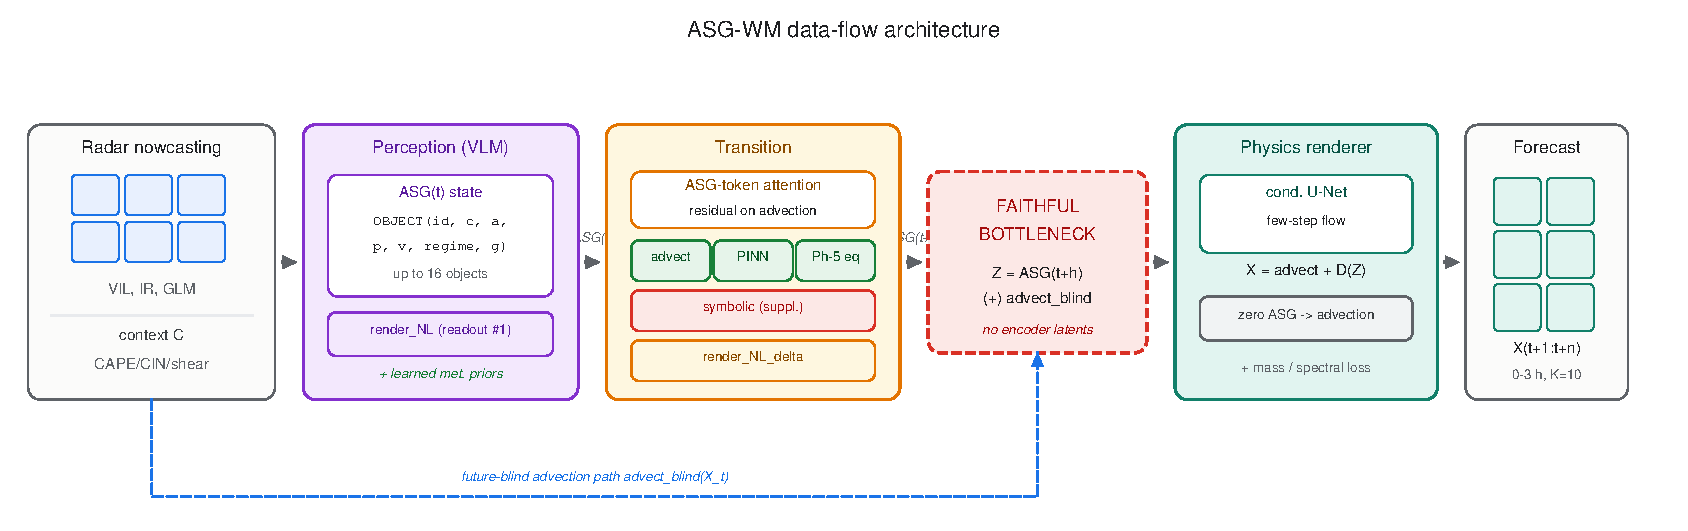
\includegraphics[width=\linewidth]{fig_architecture.pdf}
\caption{\textbf{ASG-WM data-flow architecture.}
Left to right: (\emph{Inputs}) a radar--satellite history $X_{t-k:t}$, gridded context $C$, and the VLM curriculum prompt (AFD text is training-time only; no human text at inference).
(\emph{Stage~A}) a QLoRA VLM encodes the sequence into the structured Atmospheric Scene Graph $\text{ASG}_t$ and a grammar-constrained NL readout, drawing on curriculum-learned seasonal/geographic/diurnal/synoptic priors.
(\emph{Stage~B}) a transition transformer advances the state to $\text{ASG}_{t+h}$ as a residual on advection, with governing-equation injection (differentiable advection operator, PINN continuity loss), an optional supplementary symbolic admissibility check, and a downstream NL readout $\texttt{render\_NL\_delta}(\text{ASG}_t, \text{ASG}_{t+h})$.
(\emph{Bottleneck}) the renderer receives only $Z = \text{ASG}_{t+h} \oplus \texttt{advect\_blind}(X_t)$---no encoder latents or skip connections.
(\emph{Stage~C}) a few-step latent rectified-flow renderer produces the forecast sequence as $\texttt{advect\_blind}(X_t) + \Delta(Z)$, so zeroing the ASG collapses the forecast to advection.}
\label{fig:arch}
\end{figure*}

\begin{enumerate}[leftmargin=*,nosep]
\item \textbf{Observe.}
Stage~A's VLM visual encoder reads a multi-channel radar--satellite sequence $X_{t-k:t}$ (VIL, IR069, IR107, GLM) together with physical context $C$ (CAPE, CIN, shear, PWAT from HRRR/ERA5) and NWS AFD synoptic text.
No human-supplied reasoning prompt is provided at inference.

\item \textbf{Identify.}
The VLM processes the observation and performs \emph{per-frame} storm-cell identification.
The five-phase curriculum (Section~\emph{Stage~A}: Ph-1 VQA grounding $\to$ Ph-2 ASG-faithful prose $\to$ Ph-3 structured ASG emission $\to$ Ph-4 full CoT $\to$ Ph-5 equation-aware CoT) is a \emph{training} device that progressively teaches the VLM to reason about what is present in a frame---cell locations, intensities, regime labels, growth tendencies---and emit a structured per-frame object set.
At inference the VLM produces one identification per frame; its internal chain-of-thought constrains the output but is not itself a separate reasoning step.
The result is a sequence of frame-level object sets $\{O_{t'}\}_{t'=t-k}^{t}$.

\item \textbf{Track.}
An explicit lightweight tracker links per-frame object sets from Step~Identify across the $k$-frame observation history into continuous trajectories via nearest-centroid association within a gating radius.
Each trajectory accumulates centroid positions, area, and peak intensity over time; from these the tracker derives a per-object velocity vector from multi-frame centroid displacement (more reliable than single-frame centroid differences), a track age that distinguishes true initiations (age\,$<$\,10\,min) from advecting cells, and a trajectory-length confidence.
The tracker outputs the trajectory-enriched Atmospheric Scene Graph $\text{ASG}_t$---a set of \texttt{OBJECT} tokens with stable cross-frame IDs, serialised as:
\[
\texttt{OBJECT}(id,\; c_y,\; c_x,\; a,\; p,\; v_y,\; v_x,\; r,\; g,\; \hat{c}).
\]
A constrained-grammar decoder prevents syntactic errors.
Separating Identification (spatial, single-frame) from Tracking (temporal, multi-frame) means the VLM's training target is pure spatial perception, while temporal reasoning---where did this object come from, and how fast is it moving?---is handled by a dedicated, inspectable, deterministic module.

\item \textbf{Analyze.}
Stage~B's Transition Transformer advances the trajectory-enriched world model from $\text{ASG}_t$ to $\text{ASG}_{t+h}$ using three governing-equation injection points:
(a)~a differentiable semi-Lagrangian advection operator in Stage~B ($\partial\phi/\partial t + \mathbf{v}\!\cdot\!\nabla\phi = 0$);
(b)~a PINN-style mass-conservation residual in Stage~B ($\partial g/\partial t + \nabla\!\cdot\!(g\mathbf{v}) \approx 0$);
and (c)~equation-aware \emph{training} prompts in Stage~A Ph-5 that ground perception on the advection and growth--decay relations.
Because Stage~B receives motion vectors derived from multi-frame track displacement, its task is pure dynamics prediction---\emph{how will these objects evolve?}---rather than the harder joint problem of tracking and prediction.
After predicting $\text{ASG}_{t+h}$, readout~\#2 is computed as $\texttt{render\_NL\_delta}(\text{ASG}_t, \text{ASG}_{t+h})$---a deterministic, grammar-faithful template render of the transition, not a freeform language-model output from Stage~B (Definition~\ref{def:reasoning}).
The Information Bottleneck objective trains the ASG to be a minimal sufficient statistic:
\[
\mathcal{L}_\text{IB} = \beta\,I(\text{ASG};\,X_{t-k:t}) - I(\text{ASG};\,X_{t+1:t+n}).
\]

\item \textbf{Nowcast.}
Stage~C's physics renderer materialises the forecast field exclusively from the bottleneck variable
$Z = [\,\text{ASG}_{t+h} \oplus \texttt{advect\_blind}(X_t)\,]$
as $\hat{X}_{t+h} = \texttt{advect\_blind}(X_t) + \Delta(Z)$,
where $\Delta(Z)$ is a residual produced by a rectified-flow generator conditioned solely on $Z$.
No encoder latents or radar history beyond $Z$ reach Stage~C, making the structured state causally load-bearing by construction rather than by assertion.
\end{enumerate}

\subsection*{Data}

\textbf{Primary benchmark.}
We train and evaluate primarily on SEVIR (Storm EVent ImageRy)~\cite{veillette2020sevir}, a publicly available dataset of US/CONUS storm events with co-registered multi-channel observations: vertically integrated liquid (VIL) radar composite at $384{\times}384$ spatial resolution and 1\,km per pixel, 5-min temporal sampling; GOES-16 IR channel IR069 (6.9\,\textmu m water vapour) and IR107 (10.7\,\textmu m thermal IR); and Geostationary Lightning Mapper (GLM) flash-extent density.
SEVIR provides 10,000 storm events of 4\,h duration.
For \emph{training} we draw a subset of $\approx$2,500 precipitating events using DGMR-style importance sampling~\cite{ravuri2021dgmr}: an event is retained if at least 10\,\% of pixels exceed the light-precipitation threshold in at least half of its frames, which removes near-clear-sky sequences while preserving isolated and sparse convection.
We deliberately keep this filter mild to avoid biasing against sparse/isolated initiation; all \emph{evaluation} uses the standard, unfiltered SEVIR test split, and we report the test-set precipitation-coverage distribution and per-regime frequencies in the Supplementary Information so that the (precipitation-heavier) training distribution is explicit.
All SEVIR data are accessed from AWS Open Data (bucket \texttt{s3://sevir}) at no cost.

\textbf{Physical context.}
CAPE, CIN, 0--6\,km vertical wind shear, and precipitable water (PWAT) are co-located from two sources: the NOAA High-Resolution Rapid Refresh (HRRR) model~\cite{noaa_hrrr} at 3\,km over CONUS (AWS Open Data), used for the SEVIR/CONUS training domain; and ARCO-ERA5 reanalysis~\cite{carver2023arco} (Google Cloud public bucket \texttt{gs://gcp-public-data-\allowbreak{}arco-era5}), for global coverage in cross-region experiments.
Topography is provided by the Copernicus DEM GLO-30~\cite{copernicus_dem} at 30\,m resolution, reprojected to the SEVIR grid as a static auxiliary channel.
Context fields are pre-extracted at each event's bounding box and temporal extent, cached to a persistent cloud bucket, and reused across all training runs; this pre-computation runs once on CPU and requires no GPU time.

\textbf{Meteorological text (training-time only).}
NWS Area Forecast Discussions (AFDs)~\cite{iem_afd} are retrieved from the Iowa Environmental Mesonet text-product archive and, for each training event, matched to the most recent AFD issued \emph{before} event onset.
AFDs are used \emph{exclusively as a training-time grounding signal} that teaches the VLM meteorological vocabulary and reasoning patterns; they are not provided at inference.
At inference the model operates from imagery and gridded context alone, with no human-supplied text---preserving the ``no human text at inference'' property and eliminating any concern that narrative text could leak observational references.
Because matched AFDs predate event onset they cannot in any case contain future information; restricting them to training is the stricter, cleaner choice.
Extreme-event grounding uses the NOAA Storm Events Database~\cite{noaa_storm_events} for selecting and validating high-impact training events.

\textbf{Cross-region benchmark.}
For the cross-region generalization experiments, we use [HKO-7~\cite{shi2017trajgru} / MeteoNet~\cite{larvor2020meteonet}], withheld from all SEVIR training and used for zero-shot and light-fine-tuning evaluation only.

\subsection*{Data Processing}

All preprocessing is deterministic, runs once on CPU, and is cached to a persistent bucket so it is never recomputed across the resumable training sessions (released as \texttt{scripts/00\_download\_data.py} and \texttt{01\_autolabel.py}).

\textbf{Channels and normalisation.} The four observation channels (VIL, IR069, IR107, GLM) are stacked per frame. VIL is clipped to its valid range and mapped to a reflectivity-like scale; IR brightness temperatures and GLM flash-extent density are each standardised to zero mean and unit variance using training-set statistics. Context scalars (CAPE, CIN, shear, PWAT) and the DEM are normalised the same way.

\textbf{Spatiotemporal windowing.} Events are cut into sliding windows of $k{+}1{=}13$ input frames ($\approx$60\,min of history) and $n{=}36$ target frames (the 0--3\,h horizon) at the native 5-min, 1\,km, $384{\times}384$ resolution; the transition horizon $h$ indexes a target frame. The renderer trains on $128{\times}128$ crops in the $8\times$-downsampled VAE latent (Stage~C).

\textbf{Context co-location and regridding.} HRRR (3\,km) and ARCO-ERA5 fields are bilinearly regridded to the SEVIR 1\,km grid at each event's bounding box and time; the Copernicus DEM (30\,m) is reprojected once to the same grid as a static channel. Per-event slices are cached.

\textbf{Future-blind advection.} The bypass field $\texttt{advect\_blind}(X_t)$ (Equation~\ref{eq:bottleneck}) is a semi-Lagrangian extrapolation of $X_t$ using a pysteps optical-flow field computed exclusively from $X_{\le t}$; it is precomputed and cached, and is the only kinematic signal that reaches Stage~C alongside the predicted ASG.

\textbf{Curation and sampling.} Training windows are rainy-oversampled with the mild filter defined above ($\ge$10\,\% rainy pixels in $\ge$50\,\% of frames); all evaluation uses the unfiltered standard test split.

\textbf{Splits (disjoint by construction).} Four disjoint partitions prevent leakage and selection bias: a \emph{training} set; a \emph{validation} split for model/hyperparameter selection and the Phase-3 gate; a hand-labelled \emph{gold} subset ($\approx$300 events) held out for ASG-accuracy only (Result~C-iv); and the standard SEVIR \emph{test} split for all skill metrics. The cross-region set is withheld entirely from SEVIR training.

\subsection*{Atmospheric Scene Graph Auto-Labeling}

The ASG is automatically labeled from the SEVIR VIL frames using pysteps~\cite{pulkkinen2019pysteps}, a CPU-side, zero-GPU pipeline that requires no manual annotation at training scale.

\begin{enumerate}[leftmargin=*,nosep]
    \item \textbf{Motion estimation.} Lucas-Kanade / VET optical flow is applied to consecutive VIL frames to produce per-pixel motion vectors. The same advection field is used as the future-blind path in Stage~C (Equation~\ref{eq:bottleneck}).
    \item \textbf{Cell identification (per-frame).} Watershed segmentation identifies storm-object regions above a connectivity threshold in each frame independently, producing a per-frame list of cells with centroid, area, and peak intensity. This mirrors the \emph{Identify} step of the five-step framework: purely spatial, no temporal context.
    \item \textbf{Tracking (cross-frame association).} Greedy nearest-centroid association links per-frame cells into temporal tracks, assigning stable IDs. Per-object motion vectors are derived from multi-frame centroid displacement over each track; track age governs initiation detection. This is the \emph{Track} step: deterministic, inspectable, no learned parameters.
    \item \textbf{Regime and tendency labeling (\emph{Analyze}).} Growth-decay scalar $g_t = \mathrm{d}(\text{peak\,VIL})/\mathrm{d}t$ is estimated from a 15-min track window. Regime is assigned as: initiation (track age $<$\,10\,min and area increasing), growth (VIL and area both increasing), decay (VIL and area both decreasing), or steady (otherwise).
    \item \textbf{Context co-location.} HRRR/ERA5 fields and DEM are spatially interpolated to each object centroid and attached as per-object context attributes to the ASG.
    \item \textbf{Natural-language rationale.} A deterministic template function $\texttt{render\_NL}(\text{ASG})$ emits a prose description asserting only facts present in the ASG (directional motion, regime label, intensity class, growth tendency sign). The template output is optionally paraphrased by a general-purpose instruction-tuned LLM for fluency, after which an automated assertion extractor parses the paraphrase and rejects it if it introduces any claim not entailed by the ASG, guaranteeing the prose adds no information beyond the structured state.
\end{enumerate}

Auto-labels are validated against a hand-labelled gold subset of approximately 300 events annotated independently by two domain scientists; the gold subset is held out from all fine-tuning and used only for ASG-accuracy evaluation (Result C-iv).
The pysteps tracking algorithm and its parameterisation are described fully in~\cite{pulkkinen2019pysteps}.

\subsection*{Stage A: Observation and Identification}

In the five-step reasoning flow, Stage~A covers \emph{Observe} (reading the raw multi-channel inputs) and \emph{Identify} (per-frame storm-cell classification); the explicit tracker that follows is the \emph{Track} step and is described in the next subsection.

A small VLM---SmolVLM-2.2B~\cite{marafioti2025smolvlm} or Qwen2.5-VL-3B~\cite{bai2025qwen25vl}, selected by Phase-3 ASG F1 on a disjoint validation split (\emph{not} the gold subset, which is reserved for the accuracy evaluation of Result~C-iv)---is fine-tuned with QLoRA~\cite{dettmers2023qlora} (NF4 4-bit base, LoRA rank $r=16$, $\alpha=32$) to perform per-frame storm-cell identification from the multi-channel input.
The backbone is frozen; only LoRA adapters~\cite{hu2022lora} and the modality projection layer are trained.
Multi-channel input frames (VIL\,+\,IR069\,+\,IR107\,+\,GLM) are tiled to the VLM's native patch size ($384{\times}384$); physical context scalars and equation-aware text are provided in the system prompt.

\textit{ASG grammar.}
The ASG serializes to a fixed, machine-parseable token grammar:
\[
\texttt{OBJECT}(id,\; c_y,\; c_x,\; a,\; p,\; v_y,\; v_x,\; r,\; g,\; \hat{c}),
\]
where $c_y, c_x$ are centroid coordinates (grid units), $a$ is area (km$^2$), $p$ is peak VIL (dBZ), $v_y, v_x$ are motion components (km\,h$^{-1}$), $r\in\{\text{init},\text{grow},\text{decay},\text{steady}\}$, $g$ is the growth scalar, and $\hat{c}\in[0,1]$ is perception confidence.
Constrained decoding (lm-format-enforcer) restricts the vocabulary at ASG token positions, preventing syntactic errors without modifying model weights.
Beyond the scalar confidence $\hat{c}$, the grammar admits optional per-attribute spreads $(\sigma_{c},\sigma_{v},\sigma_{g})$ on centroid, motion, and growth; in the present model these are emitted but the transition is deterministic, and a fully probabilistic ASG---predictive distributions or ensemble weights per object, enabling explicit multi-modal futures---is identified as future work (Discussion).
The natural-language description is generated by $\texttt{render\_NL}(\text{ASG})$ and cross-checked against the parsed ASG at inference; assertions absent from the ASG are suppressed.

\textit{Five-phase curriculum.}
Stage-A training follows five sequential phases, each fine-tuning from the prior checkpoint, following the VQA-to-CoT curriculum principle established in the Skew-T VLM~\cite{lee2025skewt}.
All five phases train \emph{per-frame spatial perception}---the \emph{Identify} step; temporal reasoning is the Tracker's responsibility and is not part of Stage-A training:
(1)~Visual VQA grounding on procedurally generated question--answer pairs (intensity, count, spatial, and tendency queries derived from single-frame auto-ASG labels);
(2)~ASG-faithful prose generation using the $\texttt{render\_NL}$ template, LLM-polished for fluency;
(3)~Structured ASG emission from a single frame (Phase-3 gate: ASG F1\,$\ge$\,0.70 on the validation split; this threshold is fixed from Tier-0 experiments, in which regime-label noise above $1-\text{F1}\approx0.30$ destabilised transition-transformer training, so $0.70$ is the minimum perception quality at which Stage~B converges reliably);
(4)~Full chain-of-thought reasoning (observation rationale\,$\to$\,ASG$_t$\,$\to$\,transition rationale\,$\to$\,ASG$_{t+h}$, trained as a single completion using the Tracker-produced $\text{ASG}_t$ as context, so the VLM learns consistent language about trajectories it receives as input rather than having to infer them);
(5)~Equation-aware CoT, with governing equations (advection, continuity, growth-decay parameterization) stated in the system prompt and an equation-grounding check on the training rationale.
The Phase-5 checkpoint is the Stage-A deliverable used to initialize Tier-2 training.

\subsection*{Explicit Tracker (Track Step)}

The tracker is a lightweight, deterministic module (no learned parameters in the initial design) that operates between Stage~A and Stage~B.
It takes the per-frame object sets $\{O_{t'}\}$ produced by Stage~A and links them into trajectories via greedy nearest-centroid association with a configurable gating radius (default $\approx$6\,\% of the domain diagonal).
From each trajectory it derives:
(i)~a stable object ID, consistent across the $k$-frame window;
(ii)~a velocity vector $(\hat{v}_y, \hat{v}_x)$ from mean per-step centroid displacement over the track (more accurate than single-frame differences, especially for slow-moving cells);
(iii)~a track age (in frames) that distinguishes true initiations from advecting cells for the regime labeler;
and (iv)~a trajectory-length confidence that augments the VLM's per-attribute $\hat{c}$.
These are assembled into the trajectory-enriched $\text{ASG}_t$ in the grammar above and passed to Stage~B.
Because the tracker is deterministic and inspectable---its associations can be visualised as track lines---this step can be audited and corrected independently of the neural modules.
A learned association module (e.g.\ a learned IoU threshold or appearance embedding) is identified as a natural future extension.

\subsection*{Stage B: Analysis (Transition Transformer)}

A small transformer (10--50\,M parameters) over ASG token sequences predicts $\text{ASG}_{t+h}$ from $\text{ASG}_t$ and physical context tokens.
Three governing-equation injection points constrain the dynamics without adding parameters:

\begin{enumerate}[leftmargin=*,nosep]
    \item \textbf{Differentiable advection operator.} Object centroids and the growth-decay field are advanced by a semi-Lagrangian warp using the ASG motion vectors; the network predicts the \emph{residual} on top of this advection, so the linear-motion baseline is built in.
    \item \textbf{PINN-style residual losses~\cite{raissi2019pinn}.} A mass-conservation residual on the growth field ($\partial g / \partial t + \nabla \cdot (g\mathbf{v}) \approx 0$) and a motion-field smoothness residual penalise equation violation on the predicted state.
    \item \textbf{Equation-aware training prompts (Stage~A, Ph-5).} The governing relations (advection equation $\partial\phi/\partial t + \mathbf{v}\cdot\nabla\phi = 0$; mass conservation; growth-decay parameterisation as a function of CAPE, CIN, and shear) are stated in the VLM curriculum system prompt so perception training grounds on the equations. At inference, equation injection in the transition is via items~(1)--(2) above.
\end{enumerate}

\noindent After predicting $\text{ASG}_{t+h}$, readout~\#2 is $\texttt{render\_NL\_delta}(\text{ASG}_t, \text{ASG}_{t+h})$---a deterministic, grammar-faithful template summarising the predicted evolution (regime changes, merges/splits, initiations, dissipations).

\subsection*{The Faithful Information Bottleneck}

The renderer (Stage~C) receives as its sole input:
\begin{equation}
    Z = \bigl[\, \text{ASG}_{t+h} \;\oplus\; \texttt{advect\_blind}(X_t) \,\bigr],
    \label{eq:bottleneck}
\end{equation}
where $\texttt{advect\_blind}$ is a fixed semi-Lagrangian extrapolation of $X_t$ using the pysteps optical-flow field computed exclusively from $X_{\le t}$.
No encoder latents, no skip connections from Stage~A, and no representations of the radar history beyond $Z$ reach Stage~C.
The ASG is trained to be a minimal sufficient statistic of the radar history for the future field via the Information Bottleneck objective~\cite{tishby1999ib,alemi2017vib}:
\begin{equation}
    \mathcal{L}_\text{IB} = \beta\, I(\text{ASG};\, X_{t-k:t}) - I(\text{ASG};\, X_{t+1:t+n}).
    \label{eq:ib}
\end{equation}
Minimising $\mathcal{L}_\text{IB}$ \emph{compresses} the radar history (small $I(\text{ASG};X_{t-k:t})$, weighted by $\beta$) while \emph{retaining} predictive content (large $I(\text{ASG};X_{t+1:t+n})$); the two terms have opposite sign precisely because compression and prediction are traded off, and $\beta$ sets the operating point.
The compression term is realised through a two-level scheme: (1)~a hard structural capacity cap ($N_\text{max}{=}16$ objects; motion vectors quantised to 8\,km\,h$^{-1}$ bins; growth scalar to two significant figures; four-class categorical regime) and (2)~a soft KL-divergence penalty ($\lambda_\text{IB}{=}0.01$) on continuous attributes against a unit Gaussian prior.
A capacity audit after Tier-0 quantifies the hard-capped ASG channel capacity in bits---the cap above bounds it at $\mathcal{O}(10^2)$\,bits per frame---and confirms it is several orders of magnitude smaller than the bit-capacity of the dense visual latent it replaces; the sensitivity of skill to $\beta$ and $N_\text{max}$ is reported in the capacity study (Figure~\ref{fig:capacity}).

Because $Z$ is the \emph{only} path to the output field, zeroing $\text{ASG}_{t+h}$ \emph{must} collapse the forecast to $\texttt{advect\_blind}(X_t)$, and perturbing $\text{ASG}_{t+h}$ \emph{must} produce a field change consistent with the perturbation.
These are entailments of the architecture, tested in Result~C-i and C-ii.

\subsection*{Stage C: Nowcasting (Physics-Informed Renderer)}

The renderer operates in the latent space of a frozen Stable-Diffusion VAE ($8\times$ spatial compression;~\cite{rombach2022ldm}), operating on $128{\times}128$ spatial patches with short sequences.
The forecast is decomposed as:
\begin{equation}
    \hat{X}_{t+h} = \texttt{advect\_blind}(X_t) + \Delta(Z),
\end{equation}
where $\Delta(Z)$ is the ASG-guided residual produced by a few-step rectified-flow generator~\cite{liu2023rectifiedflow} (1--4 denoising steps) conditioned on $Z$.
This residual-on-advection structure makes the bottleneck behaviour crisp: zeroed ASG implies $\Delta\to 0$, collapsing to pure advection.
The full Tier-2 loss is:
\begin{equation}
    \mathcal{L} = \mathcal{L}_\text{render} + \lambda_1 \mathcal{L}_\text{IB} + \lambda_2 \mathcal{L}_\text{intervene} + \lambda_3 \mathcal{L}_\text{mass} + \lambda_4 \mathcal{L}_\text{nonneg} + \lambda_5 \mathcal{L}_\text{spectral} + \lambda_6 \mathcal{L}_\text{continuity},
\end{equation}
where $\mathcal{L}_\text{intervene}$ is an intervention-consistency term trained on structured ASG perturbation pairs (the field difference must match the perturbation's predicted effect); $\mathcal{L}_\text{mass}$ enforces mass-budget consistency between the ASG growth field and the rendered VIL; $\mathcal{L}_\text{nonneg}$ enforces VIL\,$\ge$\,0; $\mathcal{L}_\text{spectral}$ is a radially-averaged power-spectrum loss for realism; and $\mathcal{L}_\text{continuity}$ is the Stage-B PINN residual back-propagated through the bottleneck.
The renderer backbone is a latent U-Net (100--200\,M parameters); the DiT~\cite{peebles2023dit} alternative is evaluated in the Supplementary Information.
Ensemble members for CRPS are generated by sampling the few-step flow $K{=}10$ times.
The renderer architecture is detailed in Figure~\ref{fig:renderer}.

\begin{figure*}[ht]
\centering
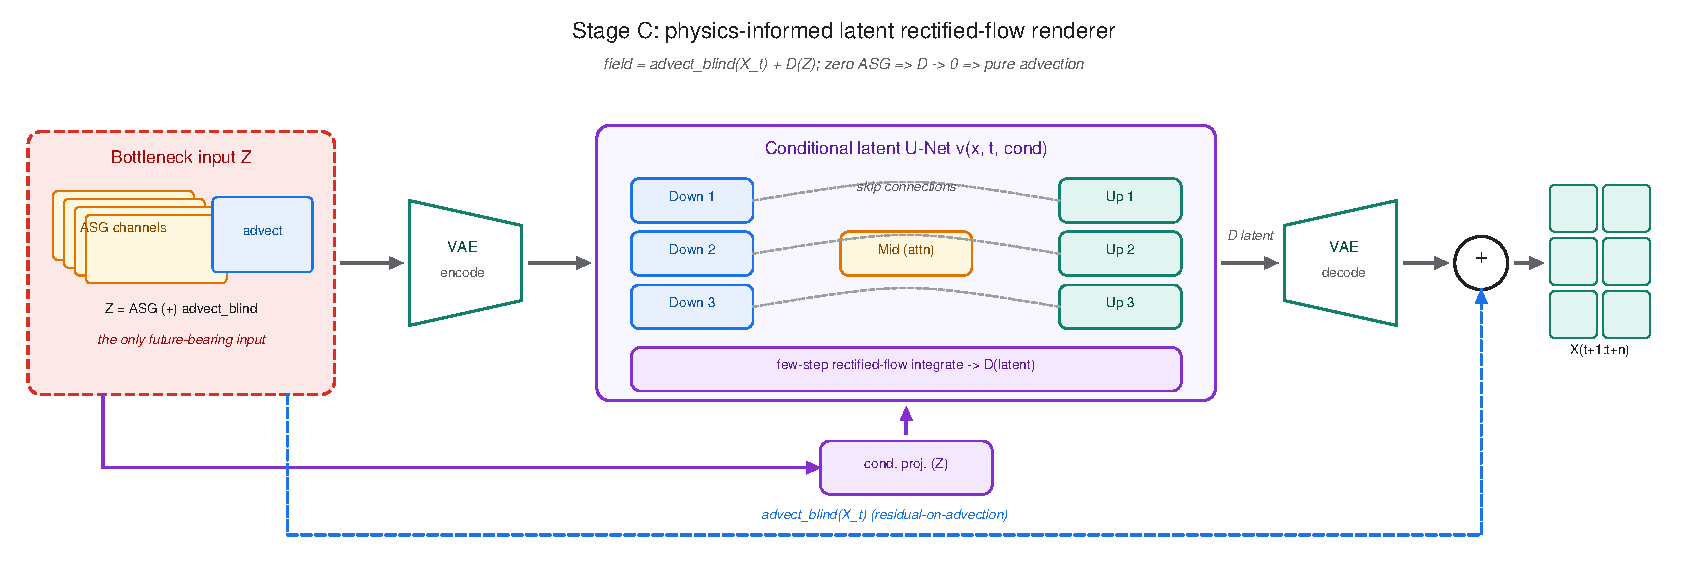
\includegraphics[width=\linewidth]{fig_renderer.pdf}
\caption{\textbf{Stage~C renderer architecture.}
The bottleneck variable $Z$---rasterised ASG guidance channels concatenated with the future-blind advection field---is the only future-bearing input.
A frozen VAE encodes the advection base to latent space; a conditional latent U-Net $v_\theta(x_\tau,\tau,\text{cond}(Z))$ with skip connections and a mid self-attention block parameterises a few-step rectified-flow velocity field, integrated in 1--4 Euler steps to a residual latent $\Delta$.
The VAE decodes $\Delta$ and it is added to the advection base, giving $\hat{X}_{t+1:t+n} = \texttt{advect\_blind}(X_t) + \Delta(Z)$; sampling the flow $K$ times yields the ensemble.
The residual-on-advection decomposition makes the faithfulness behaviour exact: zeroing the ASG channels drives $\Delta\to0$ and the forecast collapses to pure advection.}
\label{fig:renderer}
\end{figure*}

\subsection*{Governing Equations and Operators}

We collect the operators that inject physics into Stages~B and~C.

\emph{Semi-Lagrangian advection.} A field $\phi$ is advanced by back-tracing along the motion field $\mathbf{v}$ over a step $\Delta t$ and sampling the departure point,
\begin{equation}
(\mathcal{A}_{\mathbf{v}}\phi)(\mathbf{x}) = \phi\!\left(\mathbf{x} - \mathbf{v}(\mathbf{x})\,\Delta t\right),
\label{eq:advop}
\end{equation}
the discrete solution of the advection PDE $\partial_t\phi + \mathbf{v}\!\cdot\!\nabla\phi = 0$; object centroids advance as $\mathbf{c}_{t+h}=\mathbf{c}_t+\mathbf{v}\,h$. Equation~\ref{eq:advop} is both the Stage-B residual base and the future-blind path $\texttt{advect\_blind}(X_t)=\mathcal{A}_{\mathbf{v}_{\le t}}X_t$, whose flow $\mathbf{v}_{\le t}$ is estimated from $X_{\le t}$ only.

\emph{Continuity / mass conservation.} The growth field obeys $\partial_t g + \nabla\!\cdot\!(g\mathbf{v})\approx 0$; the Stage-B PINN residual penalises its violation,
\begin{equation}
\mathcal{R}_\text{cont} = \big\|\,(g_{t+h}-g_t)/h + \nabla\!\cdot\!(g_t\mathbf{v})\,\big\|_2^2 .
\label{eq:cont}
\end{equation}

\emph{Growth--decay parameterisation.} The convective tendency is forced by the environment,
\begin{equation}
g = \alpha\big(1-e^{-\mathrm{CAPE}/C_0}\big)\,e^{-\mathrm{CIN}/I_0}\,\sigma(\beta S),
\label{eq:growth}
\end{equation}
increasing with CAPE, suppressed by CIN, and organised by $0$--$6$\,km shear $S$ ($\sigma$ logistic; $\alpha,C_0,I_0,\beta$ fit on the training split).

\emph{Rectified-flow renderer.} The ASG-guided residual latent $z_1=\mathcal{E}(\Delta)$ is transported from noise $z_0\sim\mathcal{N}(0,\mathbf{I})$ along the linear path $z_\tau=(1-\tau)z_0+\tau z_1$ with constant target velocity $z_1-z_0$; the velocity network is trained by
\begin{equation}
\mathcal{L}_\text{render} = \mathbb{E}_{\tau,z_0,Z}\big\|\,v_\theta(z_\tau,\tau,Z) - (z_1-z_0)\,\big\|_2^2 ,
\label{eq:rf}
\end{equation}
and sampled by integrating $\dot z = v_\theta(z,\tau,Z)$ over $\tau\in[0,1]$ in $1$--$4$ Euler steps, giving $\hat{X}_{t+h}=\texttt{advect\_blind}(X_t)+\mathcal{D}(z_1)$.

\emph{Intervention consistency.} For a structured ASG perturbation $\delta$ with predicted field effect $\mathcal{T}_\delta$ (the entailment of Definition~\ref{def:faith}),
\begin{equation}
\mathcal{L}_\text{intervene} = \mathbb{E}_{\delta}\big\|\,[\mathcal{R}(\mathrm{do}(A\!\to\!A_\delta),B)-\mathcal{R}(A,B)] - \mathcal{T}_\delta\,\big\|_2^2 ,
\label{eq:intervene}
\end{equation}
which trains the renderer to be causally responsive to the state and supplies the paired passes scored in Result~C-i.

\emph{Capacity in bits.} With an $N_\text{max}$-object budget and per-attribute quantisation, the ASG channel capacity is bounded by
\begin{equation}
C_\text{ASG} \le N_\text{max}\sum_{a}\log_2 L_a \;\ll\; C_\text{in} = H\,W\,k\,\log_2 L_\text{px},
\label{eq:capbits}
\end{equation}
where $L_a$ is the level count of attribute $a$ and $L_\text{px}$ the per-pixel level count; the audit confirms $C_\text{ASG}\ll C_\text{in}$ before any Tier-2 run (non-vacuous bottleneck).

\subsection*{Training Recipe}

Training proceeds in three tiers to stage the thesis-critical experiments and minimise A100 session cost.

\textbf{Tier 0} (L4-24\,GB, \$0): The ASG transition transformer is trained on cached pysteps labels without VLM involvement; a deterministic renderer is trained on oracle ASGs.
Gate: the system must beat persistence and pysteps/S-PROG advection on object-evolution metrics (position error, regime-transition accuracy, growth-decay sign) before any VLM or flow-renderer training begins.
This is a publishable de-risking result that can be reported independently.

\textbf{Tier 1} (L4-24\,GB, \$0): Five-phase VLM curriculum (Section on Stage~A).
Knowledge-source ablations are run from Phase-4 and Phase-5 checkpoints.
Total curriculum time: $\approx$9--18\,h across checkpoint-resumed sessions; Phase-3 gate ($\text{F1}\ge 0.70$) is the hard decision point.

\textbf{Tier 2} (A100-40\,GB, 2--3 sessions $\times$ $<$12\,h): End-to-end coupling (Stage-A backbone frozen in 4-bit, low learning rate $\le$$10^{-5}$) plus rectified-flow renderer with intervention-consistency training; ensemble generation; cross-region fine-tuning/evaluation.
Each session resumes from a checkpoint in a persistent cloud bucket; all pre-computed artefacts (ASG labels, context slices, frozen visual features, future-blind advection fields) are cached at the outset and reused across sessions.

\subsection*{Evaluation}

Verification follows established practice~\cite{jolliffe2012forecast}.
From the contingency table at a reflectivity threshold $\theta$ (counting hits TP, false alarms FP, misses FN, correct negatives TN over $\hat{X},X \gtrless \theta$), the Critical Success Index and Heidke Skill Score are
\begin{equation}
\mathrm{CSI}=\frac{\mathrm{TP}}{\mathrm{TP}+\mathrm{FP}+\mathrm{FN}},\quad
\mathrm{HSS}=\frac{2(\mathrm{TP}\,\mathrm{TN}-\mathrm{FP}\,\mathrm{FN})}{(\mathrm{TP}{+}\mathrm{FN})(\mathrm{FN}{+}\mathrm{TN})+(\mathrm{TP}{+}\mathrm{FP})(\mathrm{FP}{+}\mathrm{TN})}.
\label{eq:csi}
\end{equation}
The Fractions Skill Score over $n{\times}n$ neighbourhoods compares fractional coverages $p_f,p_o$, $\mathrm{FSS}=1-\overline{(p_f-p_o)^2}/(\overline{p_f^2}+\overline{p_o^2})$; the ensemble CRPS for $K$ members is
\begin{equation}
\mathrm{CRPS}=\frac{1}{K}\sum_{k}|X_k-X| - \frac{1}{2K^2}\sum_{k,k'}|X_k-X_{k'}|.
\label{eq:crps}
\end{equation}
All metrics are computed on the standard SEVIR test split withheld from training.
Heavy-precipitation thresholds are the primary reporting target; light thresholds are secondary.
Reliability diagrams are reported alongside CRPS; LPIPS and PSD are reported to rule out over-smoothed skill artefacts.
For the faithfulness suite (Result~C), we report: intervention-consistency score; bottleneck-ablation CSI and CRPS under four ASG conditions; conditional MI for the leakage audit; and ASG F1, motion angular error, and regime accuracy for ASG-accuracy evaluation.
Text-overlap scores (BLEU~\cite{papineni2002bleu}, ROUGE~\cite{lin2004rouge}) against AFD text are reported as secondary metrics only; lead metrics are faithfulness measures (C) and regime-stratified skill (B).

% ===================================================================
\section*{Acknowledgements}
% ===================================================================

\noindent [To be completed upon study conclusion.]

% ===================================================================
\section*{Author Contributions Statement}
% ===================================================================

\noindent [To be completed.]

% ===================================================================
\section*{Additional Information}
% ===================================================================

\noindent \textbf{Competing interests:} The authors declare no competing interests.

\noindent \textbf{Data and code availability:} The SEVIR dataset is available at \texttt{s3://sevir} (AWS Open Data). HRRR data are available at \texttt{s3://noaa-hrrr-bdp-pds}. ARCO-ERA5 is at \texttt{gs://gcp-public-data-arco-era5}. AFD archives are available via the Iowa Environmental Mesonet API. The ASG auto-labeling pipeline, model weights, and evaluation code will be released at [repository URL].

% ===================================================================
\section*{Supplementary: VLM Curriculum Prompts}
% ===================================================================

\noindent The Stage-A five-phase curriculum uses the prompt templates below (reproduced verbatim from the released code, \texttt{asgwm/models/prompts.py}). Placeholders \texttt{\{context\}}, \texttt{\{grammar\}}, \texttt{\{equations\}}, and \texttt{\{question\}} are filled at runtime: \texttt{\{context\}} renders the co-located environmental scalars (CAPE/CIN/shear/PWAT/DEM), \texttt{\{grammar\}} the fixed ASG grammar, and \texttt{\{equations\}} the governing-equation block (Phase~5 only). The structured output obeys the grammar exactly; the natural language is a constrained render of that state.

\noindent\textbf{ASG grammar block} (\texttt{\{grammar\}}):
\begin{lstlisting}
Emit the Atmospheric Scene Graph (ASG) in this exact grammar, one line each:
GLOBAL(regime=<init|grow|decay|steady>, n_objects=<int>)
OBJECT(id=<int>, cy=<float>, cx=<float>, area=<float_km2>, peak=<float_dBZ>,
       vy=<float_kmh>, vx=<float_kmh>, regime=<init|grow|decay|steady>,
       growth=<float>, conf=<float_0_1>)
One GLOBAL line, then one OBJECT line per storm cell.
Units are fixed by position; emit no other text.
\end{lstlisting}

\noindent\textbf{Governing-equation block} (\texttt{\{equations\}}, injected at Phase~5):
\begin{lstlisting}
Governing equations (reason WITH these, not prose alone):
1. Advection (Lagrangian form): dphi/dt + v . grad(phi) = 0 -- precipitation
   features are transported by the motion vector v=(vy,vx); centroids advance
   along v over the horizon.
2. Continuity / mass-conservation: the integrated VIL tendency balances flux
   convergence -- growth requires net convergence, decay net divergence.
3. Growth-decay parameterization: the convective tendency g is forced by the
   environment -- it increases with CAPE, is suppressed by CIN, and is organized
   by vertical wind shear. Use the context scalars (cape, cin, shear, pwat).
\end{lstlisting}

\noindent\textbf{Phase 1 --- Visual VQA grounding:}
\begin{lstlisting}
You are a radar nowcasting assistant. Look at the provided radar/satellite frames
and answer the question with a short, factual response grounded only in what is
visible. Do not speculate beyond the imagery.
{context}
Question: {question}
Answer:
\end{lstlisting}

\noindent\textbf{Phase 2 --- ASG-faithful object description:}
\begin{lstlisting}
You are a meteorological analyst. Describe the precipitation scene in the provided
radar/satellite frames in natural language. State only facts grounded in the scene:
the number of cells, the overall regime, each cell's intensity class
(light/moderate/heavy), its compass direction of motion, and its growth tendency
(intensifying/weakening/steady). Do not invent specific numeric values.
{context}
Description:
\end{lstlisting}

\noindent\textbf{Phase 3 --- Structured ASG output (gate: F1 $\ge$ 0.70):}
\begin{lstlisting}
You are a radar nowcasting perception model. From the provided radar/satellite
frames and the environmental context, identify the storm cells and emit the
current Atmospheric Scene Graph.
{context}
Valid regimes: init, grow, decay, steady.
{grammar}
ASG:
\end{lstlisting}

\noindent\textbf{Phase 4 --- Chain-of-thought (state before rationale):}
\begin{lstlisting}
You are a meteorological reasoning model performing radar nowcasting. From the
provided radar/satellite frames and environmental context, reason about the current
scene and its evolution over the forecast horizon.
{context}
Valid regimes: init, grow, decay, steady.
{grammar}
Produce your output in this exact order:
OBSERVATION: <one-paragraph rationale describing the present scene>
ASG_T:
<the current ASG in grammar>
TRANSITION: <one-paragraph rationale for how the scene evolves over the horizon>
ASG_TH:
<the forecast ASG in grammar>
Emit the ASG state lines before each rationale section as labelled above.
\end{lstlisting}

\noindent\textbf{Phase 5 --- Equation-aware chain-of-thought:}
\begin{lstlisting}
You are a physics-grounded meteorological reasoning model performing radar
nowcasting. Use the governing equations below explicitly in your reasoning.
{equations}
{context}
Valid regimes: init, grow, decay, steady.
{grammar}
Produce your output in this exact order:
OBSERVATION: <present-scene rationale>
ASG_T:
<the current ASG in grammar>
TRANSITION: <forecast rationale that references the relevant physical quantities:
the motion vector (advection), continuity/convergence, and the growth forcing
from CAPE/CIN/shear>
ASG_TH:
<the forecast ASG in grammar>
\end{lstlisting}

\bibliography{references}

\end{document}
